\documentclass[a4paper, 11pt]{article}

%--------------------------------------------------------------------
%--- Title, author, date
%--------------------------------------------------------------------

\newcommand{\docauthor}{Martins Bruveris}
\newcommand{\docdate}{2016 $|$ November $|$ 14}
\newcommand{\docclass}{MA2712}
\newcommand{\doctitle}{Problems Part II}

%--------------------------------------------------------------------
%--- Input custom header
%--------------------------------------------------------------------

%--------------------------------------------------------------------
%--- Notes to myself
%--------------------------------------------------------------------

% TODO: Tautasdziesma
% TODO: Figure out how vertical space works in title page
%       Clean up code for title page
% TODO: Add section numbers to pdf bookmarks
% TODO: Change document class to book to have two parts
%       Part 1 - problems
%       Part 2 - solutions
%       Both in one document
% TODO: Work on page geometry

% Need gnuplot to compile this
% TODO: Add id to plots, so we can compile without gnuplot,
%       see TikZ manual p.329.
% TODO: Change figuretable to use tabu
%       Avoid globally resetting \tabcolsep
% TODO: Tables for local extrema look bad
% 
% TODO: Sect. 10, choose better functions to integrate over
%       rectangles
% TODO: Check for consistent usage of alignenum
% 
%--------------------------------------------------------------------
%--- Loading packages
%--------------------------------------------------------------------

\PassOptionsToPackage{dvipsnames}{xcolor} % Is loaded by TikZ                                

\usepackage{amsmath,amsthm,textcomp}

\usepackage[charter,expert]{mathdesign}   % Bitstream Charter font, 
                                          % as recommended by Aleksey
\usepackage[scaled=.96,osf]{XCharter}     % Matches the size used in math
\usepackage{microtype}                    % Typographical improvements
\usepackage{bm}

\usepackage[T1]{fontenc}  % These three packages load Times fonts
% \usepackage{mathptmx}
% \usepackage{tgtermes} 

% \usepackage{newtxtext}  % Other fonts to consider
% \usepackage{newtxmath}

\usepackage[utf8]{inputenc}
\usepackage{graphicx}

\usepackage{enumitem}                     % Customize lists
% \usepackage{enumerate}                  
\usepackage{geometry}                     % Customize page geometry
% \usepackage{showframe}                    % To show page geometry
\usepackage{fancyhdr}                     % Custom headers and footers
\usepackage{lastpage}                     % To show "Page 1 / 20"

\usepackage{tikz}                         % For drawing figures

\usepackage{exsheets}                     % For problem/solution environments
\usepackage{wrapfig}                      % To let text wrap around a figure
\usepackage{adjustbox}                    % For wrapfigure inside enumerate
\usepackage{ifthen}                       % iften for defining commands
\usepackage{siunitx}                      % To typeset units
\usepackage{tabu}                         % tabu environment for tables
\usepackage{tasks}                        % tasks environment for horizontal lists
\usepackage{nth}
\usepackage[savepos]{zref}                % For align in enumerate workaround
\usepackage{etoolbox}                     % For parameter toggles
\usepackage{xcolor}                       % For red title

\usepackage[style=numeric, minnames=3,
            doi=false, url=false, isbn=false,
            firstinits=true,
            sortcites=true,
            backend=biber]{biblatex}      % For bibliographies

%--------------------------------------------------------------------
%--- Pdf options
%--------------------------------------------------------------------

\usepackage[
  pdftitle={\docclass{} -- \doctitle}, 
  pdfauthor={\docauthor},
  colorlinks=true,
  linkcolor=blue,
  urlcolor=blue,
  citecolor=blue,
  bookmarks=true,
  bookmarksopenlevel=2]{hyperref}

\usepackage[inline]{asymptote}            % For asymptote graphics

%--------------------------------------------------------------------
%--- Global page geometry and layout
%--------------------------------------------------------------------

\geometry{
%  total={210mm,297mm},
  left=25mm,
  right=25mm,
  bindingoffset=0mm, 
  top=20mm,
  bottom=20mm
}

\fancyhf{}
\renewcommand{\headrulewidth}{0.5pt}
\fancyhead[L]{\textsc{\docclass}}
\fancyhead[C]{\textsc{\doctitle}}
\fancyhead[R]{\textsc{\docdate}}
\renewcommand{\footrulewidth}{0.5pt}
\fancyfoot[L]{\textsc{\docauthor}}
\fancyfoot[C]{}
\fancyfoot[R]{\textsc{Page \thepage\ /\ \pageref*{LastPage}}}

\setlength{\headheight}{14pt} % Was necessary, warning otherwise

\fancypagestyle{firstpage}{
  \fancyhf{}
  \renewcommand{\footrulewidth}{0pt}
  \fancyfoot[L]{}
  \fancyfoot[C]{}
  \fancyfoot[R]{}
  \renewcommand{\headrulewidth}{0mm}
}

\pagestyle{fancy}

\author{\docauthor}
\date{\docdate}
\title{\docclass{} -- \doctitle}

% Custom Title
\newcommand{\linia}{\rule{\linewidth}{0.5pt}}

\makeatletter
\renewcommand{\maketitle}{
\begin{center}
\vspace{2ex}
{\huge \textsc{\@title}}
\vspace{1ex}
\\
\linia\\
\textsc{\@author} \hfill \textsc{\@date}
\vspace{4ex}
\end{center}
}
\makeatother

%--------------------------------------------------------------------
%--- Microtype settings
%--- Source: microtype documentation
%--------------------------------------------------------------------

\microtypesetup{expansion=alltext, step=1}
\microtypesetup{kerning=true}

\DeclareMicrotypeSet*[protrusion]
  { doc }
  { encoding = {*, TS1, OMS},
    family   = {rm*, tt*},
    size     = {footnotesize, small, normalsize} }
\SetProtrusion
  { encoding = OMS,
    family   = mdbch }
  { "68 = {400, },  % \langle
    "69 = { ,400} } % \rangle
\DeclareMicrotypeSet*[kerning]
  { doc }
  { encoding = T1,
    family   = blg, % typewriter font and ...
    font     = * }  % French sample in section \ref{sub:kerning}
\SetExtraKerning
  { encoding = T1,
    family   = blg }
  { _ = {100,100} } % underscores shouldn't touch

%--------------------------------------------------------------------
%--- Global parameters and commands
%--------------------------------------------------------------------

\linespread{1.2}

\everymath{\displaystyle}

% Table to typeset tikz figures; parameter is number of columns
\newenvironment{figuretable}[2][1em]
  {
    \begin{tabular}{*{#2}{c@{\hspace{#1}}}}
  }
  {
    \end{tabular}
  }

% A better solution should be found for this...
\tabcolsep=0pt

% Used to adjust vertical height for wrapfigure inside enumerate
\newlength{\strutheight}
\settoheight{\strutheight}{\strut}

\renewcommand{\labelenumi}{(\alph{enumi})} % Use letters for enumerate

\settasks{counter-format=(tsk[a])} % Use letters for tasks lists
\settasks{label-width={1.5em}}

\let\six=\si % \si is defined by package siunitx, but we use it for \sigma

% Pagebreak after each problem section
\newboolean{sectionnewpage}
\setboolean{sectionnewpage}{false}

% For printing difficulty level
\newcommand{\difficulty}[1]{(#1)}

% Bibliography
\addbibresource{bibliography.bib}

% Align in enumerate environment
% Source: tex.stackexchange.com/questions/9394
\newenvironment{alignenum}{%
  $\begin{aligned}[t]
}{%
  \end{aligned}$
}
% This one has centered formulas
% \newenvironment{alignenum}{%
%   \hfill$\begin{aligned}[t]
% }{%
%   \end{aligned}$\hfill\null
% }

\newcounter{dummy} % necessary for correct hyperlinks (to index, bib, etc.)

%--------------------------------------------------------------------
%--- Question/Solution environments
%--------------------------------------------------------------------

% From tex.stackexchange.com/questions/249455 
% to enable displaying question source
\ExplSyntaxOn
\RenewDocumentCommand{\QuestionNumber}{sm}
 {
  \IfBooleanTF{#1}
   { \exsheets_question_number:o {#2} }
   { \exsheets_question_number:n {#2} }
 }
\cs_generate_variant:Nn \exsheets_question_number:n { o }

\RenewDocumentCommand{\IfQuestionPropertyTF}{smmmm}
 {
  \IfBooleanTF{#1}
   { \exsheets_if_question_property:noTF { #2 } { #3 } { #4 } { #5 } }
   { \exsheets_if_question_property:nnTF { #2 } { #3 } { #4 } { #5 } }
 }
\cs_generate_variant:Nn \exsheets_if_question_property:nnTF { no }
\ExplSyntaxOff

% To display question source
\DeclareQuestionProperty{source}
\DeclareQuestionProperty{difficulty}

\SetupExSheets{
  question/post-body-hook={%
    \IfQuestionPropertyTF*%
      {source}%
      {\CurrentQuestionID}%
      {\strut\hfill \mbox{[\GetQuestionProperty{source}{\CurrentQuestionID}]}}%
      {}%
    } ,
  question/pre-body-hook={%
    \IfQuestionPropertyTF*%
      {difficulty}%
      {\CurrentQuestionID}%
      {{\bfseries\difficulty{\GetQuestionProperty{difficulty}{\CurrentQuestionID}}}}%
      {}%
  } 
}

\DeclareInstance{exsheets-heading}{block-nonr}{default}{
  title-post-code = {\bfseries .} ,
  attach = {
    main[l,vc]title[l,vc](0pt,0pt) ;
    main[r,vc]points[l,vc](\marginparsep,0pt)
  }
}

\DeclareInstance{exsheets-heading}{runin-nonr}{default}{
  runin = true ,
  title-post-code = {\bfseries .\space} ,
  attach = {
    main[r,vc]points[l,vc](\marginparsep,0pt)
  } ,
  join = {
    main[r,vc]title[r,vc](0pt,0pt)
  }
}

\RenewQuSolPair
  {question}[headings=margin-nr]
  {solution}[headings=runin-nonr]

%--------------------------------------------------------------------
%--- Some theorem-like environments
%--------------------------------------------------------------------

\newtheoremstyle{theoremnote}%
  {\parskip}%   Space above
  {0pt}%        Space below
  {}%           Body font
  {\parindent}% Indent amount
  {\itshape}%   Theorem head font
  {:}%          Punctuation after theorem head
  {.5em}%       Space after theorem head
  {\thmnumber{#2 }\thmname{#1}\thmnote{. #3}}%  Theorem head spec

\theoremstyle{theoremnote}
\newtheorem*{note*}{Note}

\newtheoremstyle{theoremhint}%
  {\parskip}%   Space above
  {0pt}%        Space below
  {}%           Body font
  {}% Indent amount
  {\itshape}%   Theorem head font
  {:}%          Punctuation after theorem head
  {.5em}%       Space after theorem head
  {\thmnumber{#2 }\thmname{#1}\thmnote{. #3}}%  Theorem head spec

\theoremstyle{theoremhint}
\newtheorem*{hint*}{Hint}


%--------------------------------------------------------------------
%--- Tikz setup and parameters
%--------------------------------------------------------------------

\usetikzlibrary{intersections}
\usetikzlibrary{calc}
\usetikzlibrary{math}
\usetikzlibrary{arrows.meta}
\usetikzlibrary{patterns}
\usetikzlibrary{external}        % To create standalone pdf files
 

% \tikzset{external/disable dependency files=false}
% \tikzexternalize % Activate externalization
\tikzsetexternalprefix{tmp_tikz/}
\tikzset{external/optimize command away=\asyinclude}
\tikzset{external/optimize command away=\asy} % Unclear if it will work

% Global parameters for figures
\tikzset{
  integration domain/.style = {fill=blue!30}
}

\tikzset{
  integration domain2/.style = {fill=red!30}
}

\tikzset{
  coordinate grid/.style = {color=gray!40, thin}
}

\tikzset{
  every node/.style = {font = \footnotesize}
}

% Arrowhead, mostly for coordinate axes
\tikzset{
    >={Stealth[length=2mm]}
}

% Arrowtips for vector fields; should provided \scale is defined locally
\tikzset{
  vector field/.style={
    ->, blue,
    >={Straight Barb[length={1.5pt}, width={1.5pt}]}
  },
  vector field/.default=\scale
}

\newcommand{\drawaxes}[4]{
  \draw[->,>={Stealth[length={4pt}]}]
    ({#1-0.1*(#3-#1)},0) -- ({#3+0.1*(#3-#1)},0) node[below] {$x$};
  \draw[->,>={Stealth[length={4pt}]}] 
    (0,{#2-0.1*(#4-#2)}) -- (0,{#4+0.1*(#4-#2)}) node[left] {$y$};
}

\newcommand{\drawaxeslabelled}[6]{
  \draw[->,>={Stealth[length={4pt}]}]
    ({#1-0.1*(#3-#1)},0) -- ({#3+0.1*(#3-#1)},0) node[below] {#5};
  \draw[->,>={Stealth[length={4pt}]}] 
    (0,{#2-0.1*(#4-#2)}) -- (0,{#4+0.1*(#4-#2)}) node[left] {#6};
}

\newcommand{\drawxaxis}[3][$x$]{
  \draw[->,>={Stealth[length={4pt}]}]
    ({#2-0.1*(#3-#2)},0) -- ({#3+0.1*(#3-#2)},0) node[below] {#1};
}

\newcommand{\drawyaxis}[3][$y$]{
  \draw[->,>={Stealth[length={4pt}]}] 
    (0,{#2-0.1*(#3-#2)}) -- (0,{#3+0.1*(#3-#2)}) node[left] {#1};
}

\newcommand{\drawxlabels}[2][fill]{
  \foreach \x/\xtext in {#2} {
    \ifthenelse{\equal{#1}{fill}}
    {
      \draw[shift={(\x,0)}] (0pt,{2.5pt/\scale}) -- (0pt,{-2.5pt/\scale}) 
        node[below,fill=white] {$\xtext$};
    }
    {
      \draw[shift={(\x,0)}] (0pt,{2.5pt/\scale}) -- (0pt,{-2.5pt/\scale}) 
        node[below] {$\xtext$};
    }
  }
}

\newcommand{\drawylabels}[2][fill]{
  \foreach \y/\ytext in {#2} {
    \ifthenelse{\equal{#1}{fill}}
    {
      \draw[shift={(0,\y)}] ({2.5pt/\scale},0pt) -- ({-2.5pt/\scale},0pt) 
        node[left,fill=white] {$\ytext$};
    }
    {
      \draw[shift={(0,\y)}] ({2.5pt/\scale},0pt) -- ({-2.5pt/\scale},0pt) 
        node[left] {$\ytext$};
    }
  }
}

\newcommand{\drawpoint}[1]{
 \draw[fill=white] #1 circle [radius=2.5pt/\scale];
}

% Scale of integration regions
% (extent of x-axis) * (scale) = 3.75 = 15/4

% Margin for coordinate axes: 10% in each direction

% Baseline for figure to be set at bottom edge of coordinate grid

%--------------------------------------------------------------------
%--- Global settings for Asymptote graphics
%--------------------------------------------------------------------

\def\asydir{tmp_asy}

\begin{asydef}
import palette;
import three;
import graph3;
import grid3;
import solids;

texpreamble("\usepackage[charter,expert]{mathdesign}");

triple XZplane(pair z) {return (z.x,0,z.y);}

defaultpen(fontsize(8pt));

// Materials for surface patches
// 0 .. (blue)                emphasized region
// 1 .. (grey)                nonemphasized region
// 2 .. (not drawn)
// 3 .. (light grey, trans)   nonemphasized, transparent
// 4 .. (light red, trans)    auxilary surface
material[] surface_pens =
	new material[] {lightblue+opacity(1.),
									material(diffusepen=lightgray+opacity(1.), 
													 emissivepen=gray(0.3),
													 specularpen=gray(0.2)),
									lightgrey+opacity(0.),
									lightgrey+opacity(0.8),
									red+opacity(0.2)};
material aux_surface_pen = surface_pens[4];

int emph_ind = 0;
int grey_ind = 1;
int trns_ind = 2;
int grtr_ind = 3;
int auxs_ind = 4;

// Mesh lines on surface
pen mesh_pen = black;
// Color of grid in xy-plane
pen xygrid_pen = grey;
// Color of vertical lines
pen support_lines_pen = grey;
// Mesh lines on auxilary surface
pen aux_mesh_pen = white+opacity(1);

// LEGACY NAMES
// material[] graph_colors = surface_pens;
// material[] graph_colors2 = new material[] { graph_colors[0], graph_colors[3] };
// pen graph_meshpen = mesh_pen;
// pen aux_surface_meshpen = aux_mesh_pen;

settings.prc = false;

// Settings for debugging
settings.render=1;
int resx = 20;
int resy = 20;

// Settings for pdf -- they are toggled below
// settings.render = 16;
// settings.prc = false;
// int resx = 300; // Resolution of spline surfaces
// int resy = 300;

// Problem with graphic card; if maxtile=(0,0) works, use it
// Source: tex.stackexchange.com/questions/176539/
settings.maxtile=(600, 600); 

import "../asy/ma2712.asy" as ma2712;
\end{asydef}

% Do we want high resolution?
\newif\ifasyhighres
\asyhighresfalse
\input{asy_flags}

\ifasyhighres
\begin{asydef}
settings.render = 16;
int resx = 300;
int resy = 300;
\end{asydef}
\fi

%--------------------------------------------------------------------
%--- Math Notation
%--------------------------------------------------------------------
\newcommand{\al}{\alpha} 
\newcommand{\be}{\beta} 
\newcommand{\ga}{\gamma} 
\newcommand{\de}{\delta} 
\newcommand{\ep}{\varepsilon} 
\newcommand{\ze}{\zeta} 
\newcommand{\et}{\eta} 
\renewcommand{\th}{\theta} % Already defined by T1 encoding
\newcommand{\io}{\iota} 
\newcommand{\ka}{\kappa} 
\newcommand{\la}{\lambda} 
\newcommand{\rh}{\varrho} 
\renewcommand{\si}{\sigma} % Already defined by siunitx
\newcommand{\ta}{\tau} 
\newcommand{\ph}{\varphi} 
\newcommand{\ch}{\chi} 
\newcommand{\ps}{\psi} 
\newcommand{\om}{\omega} 
\newcommand{\Ga}{\Gamma} 
\newcommand{\De}{\Delta} 
\newcommand{\Th}{\Theta}
\newcommand{\La}{\Lambda} 
\newcommand{\Si}{\Sigma} 
\newcommand{\Ph}{\Phi} 
\newcommand{\Ps}{\Psi} 
\newcommand{\Om}{\Omega}
 
\def\inv{^{-1}} 
\def\x{\times}
\def\p{\partial} 
\def\N{{\mathbb N}}
\def\R{{\mathbb R}}
\def\exp{\operatorname{exp}}
\def\one{\mathbbm{1}}

\def\leq{\leqslant}
\def\geq{\geqslant}

\let\on=\operatorname
\let\wt=\widetilde
\let\wh=\widehat
\let\ol=\overline

\let\mb=\mathbb
\let\mc=\mathcal
\let\mf=\mathfrak

\newcommand{\ud}{\,\mathrm{d}}
\renewcommand{\vec}[1]{\bm{\mathrm{#1}}}


%--------------------------------------------------------------------
%--- Formatting commands
%--------------------------------------------------------------------

% Pagebreak after each problem section
\setboolean{sectionnewpage}{false}

% Print solutions or not
\SetupExSheets{solution/print=false}

%--------------------------------------------------------------------
%--- The document
%--------------------------------------------------------------------

\begin{document}

\maketitle
\thispagestyle{firstpage}

\tableofcontents
\newpage

\setcounter{section}{9}
\setcounter{question}{90}

\section{The Double Integral and Iterated Integrals}
\begin{question}
\SetQuestionProperties{source = {Ex. 1,2; MW, III.17.1}}
The function $g$ takes values on the rectangles as indicated in the figure below. Calculate the integral of $g$.

\begin{center}
\begin{tabu} to \linewidth {*2{X[1,c]}}
\begin{tikzpicture}[scale=0.6, baseline=0]
  \def\scale{0.6}
  % \draw[coordinate grid, step=1.] (0,0) grid (4,4);

  \drawxlabels{1/1, 4/4}
  \drawylabels{3/3, 4/4}
  \drawaxes{0}{0}{4.4}{4.4}

  \draw (1,0) -- (1,4);
  \draw (4,0) -- (4,4);
  \draw (0,3) -- (4,3);
  \draw (0,4) -- (4,4);

  \node at (0.5, 1.5) {$-2$};
  \node at (0.5, 3.5) {$0$};
  \node at (2.5, 1.5) {$1$};
  \node at (2.5, 3.5) {$3$};
\end{tikzpicture}
&
%0.9375
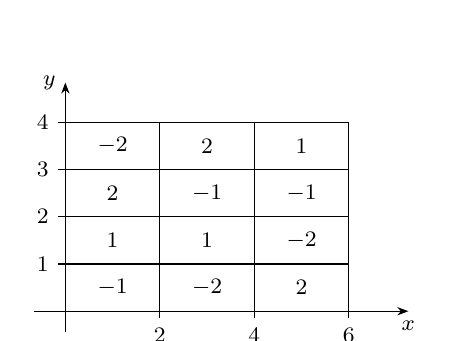
\begin{tikzpicture}[scale=0.6, baseline=(X.base)]
  \def\scale{0.6}
  \node at (0,0) (X) {};

  \drawaxes{0}{0}{6.6}{4.4}

  \foreach \x in {2, 4, 6} {
    \draw (\x, 0) -- (\x, 4);
  }

  \foreach \y in {1, 2, 3, 4} {
    \draw (0, \y) -- (6, \y);
  }

  \foreach \x/\y/\text in {1/0.5/-1, 1/1.5/1, 1/2.5/2, 1/3.5/-2,
                           3/0.5/-2, 3/1.5/1, 3/2.5/-1, 3/3.5/2,
                           5/0.5/2, 5/1.5/-2, 5/2.5/-1, 5/3.5/1} {
    \node at (\x, \y) {$\text$};
  }

  \drawxlabels{2/2, 4/4, 6/6};
  \drawylabels{1/1, 2/2, 3/3, 4/4};
\end{tikzpicture}
\\
(a) & (b)
\end{tabu}
\end{center}
\end{question}

\begin{solution}
\begin{enumerate}
\item
Denote the rectangle $D = [0,4] \x [0,4]$. Because $g$ is a step function, we can evaluate the integral as follows
\[
\iint_D g(x,y) \ud x \ud y =
-2 \cdot 3 + 1 \cdot 9 + 0 \cdot 1 + 3 \cdot 3 = 12\,.
\]
\item
Similarly to the previous exercise, let $D = [0,6] \x [0,4]$. Each smaller rectangle has the same area $2$ and therefore
\begin{align*}
\iint_D g(x,y) \ud x \ud y &=
-2 \cdot \left( -2 + 2 + 1 + 2 -1 -1 + 1 + 1 -2 -1 -2 + 2\right)
= 0\,.
\end{align*}
\end{enumerate}
\end{solution}

\begin{question}
\SetQuestionProperties{source = {Ex. 5; MW, III.17.1}}
Evaluate the iterated integrals
\begin{tasks}(2)
\task
$\displaystyle \int_0^3 \int_0^2 x^3 y \ud x \ud y$.
\task
$\displaystyle \int_0^3 \int_0^2 x^3 y \ud y \ud x$.
\end{tasks}
\end{question}

\begin{solution}
\begin{enumerate}
\item
We have
\begin{align*}
\int_0^3 \int_0^2 x^3 y \ud x \ud y
&= \int_0^3 \frac 14 x^4 y \bigg|_{x=0}^2 \ud y
= 4 \int_0^3 y \ud y = 18\,.
\end{align*}

\item
We have
\begin{align*}
\int_0^3 \int_0^2 x^3 y \ud y \ud x
&= \int_0^3 \frac 12 x^3 y^2 \bigg|_{y=0}^2 \ud x
= \int_0^3 2 x^3 \ud x = \frac{81}{2} \,.
\end{align*}
\end{enumerate}
\end{solution}

\begin{question}
\SetQuestionProperties{source = {Ex. 12, 14--16; MW, III.17.1}}
Evaluate $\displaystyle\iint_{D} f(x,y) \ud x \ud y$ for the following functions and rectangles.
\begin{tasks}(2)
\task
$f(x,y) = xy^3 e^{x^2 y^2}$; $D=[1,3] \x [1,2]$.
\task
$\displaystyle f(x,y) = xy + \frac{x}{y+1}$; $D=[1,4]\x [1,2]$.
\task
$\displaystyle f(x,y) = y^3 \cos^2 x$; $D=[-1,2]\x [0,2]$.

{\itshape Hint:} Use half-angle formulas for $\cos^2 x$.
\task
$\displaystyle f(x,y) = y^5 \sin x\, e^{y^3 \cos x}$; $D=[0,1]\x [-1,0]$.
\end{tasks}
\end{question}

\begin{solution}
\begin{enumerate}
\item
We have
\begin{align*}
\int_1^2 \int_1^3 xy^4 e^{x^2y^2} \ud x \ud y
&= \int_1^2 \frac 12 y e^{x^2y^2} \bigg|_{x=1}^3 \ud y
= \int_1^2 \frac 12 y \left( e^{9y^2} - e^{y^2}\right) \ud y \\
&= \frac{1}{36} e^{9y^2} - \frac{1}{4} e^{y^2} \bigg|_{y=1}^2
= \frac{1}{36} \left(e^{36} - e^9\right) - \frac{1}{4} \left(e^4 - e\right)\,.
\end{align*}
\item We have
\begin{align*}
\int_1^4 \int_1^2 xy + \frac{x}{y+1} \ud y \ud x
&= \int_1^4 x \ud x \int_1^2 y + \frac{1}{y+1} \ud y \\
&= \left(\left. \frac{x^2}2 \right|_{x=1}^4 \right) \left(\left. \frac{y^2}2 + \ln(y+1) \right|_{y=1}^2 \right)
= \frac {45}4 + \frac{15}2 \ln \frac 32\,.
\end{align*}
\item
We have
\begin{align*}
\int_{-1}^2 \int_0^2 y^3 \cos^2 x \ud y \ud x &=
\int_{-1}^2 \frac 14 y^4 \cos^2 x \bigg|_{y=0}^2 \ud x
= \int_{-1}^2 4 \cos^2 x \ud x 
= \int_{-1}^2 2 + 2\cos 2x \ud x \\
&= 2x + \sin 2x \bigg|_{x={-1}}^2 = 6 + \sin 2 + \sin 4\,.
\end{align*}
\item
We choose the following order of integration
\begin{align*}
\int_{-1}^0 \int_0^1 y^5 \sin x\, e^{y^3 \cos x} \ud x \ud y
&= \int_{-1}^0 -y^2 e^{y^3 \cos x} \bigg|_{x=0}^1 \ud y
= \int_{-1}^0 -y^2 e^{y^3 \cos 1} + y^2 e^{y^3}\ud y \\
&= \left.\frac{-1}{3\cos 1} e^{y^3 \cos 1} + \frac 13 e^{y^3} \right|_{y=-1}^0 \\
&= \frac 13 - \frac 1{3e} + \frac{1}{3\cos 1}\left(e^{-\cos 1} - 1\right)\,.
\end{align*}
\end{enumerate}
\end{solution}

\begin{question}
\SetQuestionProperties{source = {Ex. 19; MW, III.17.1}}
Find the volume under the graph of
\[
f(x,y) = x^3 + y^2 + 2\,,
\]
between the planes
\[
x=-1, x=1, y=1 \text{ and } y=3\,.
\]
\end{question}

\begin{solution}
The volume is given by the integral
\begin{align*}
\iint_{[-1,1]\times [1,3]} x^3 + y^2 + 2 \ud x \ud y
&= \int_{-1}^1 \int_1^3 x^3 + y^2 + 2 \ud y \ud x \\
&= \int_{-1}^1 x^3y + \frac 13 y^3 + 2y \bigg|_{y=1}^3 \ud x
= \int_{-1}^1 2x^3 + \frac{38}3 \ud x \\
&= \frac 12 x^4 + \frac{38}3x \bigg|_{x=-1}^1 = \frac{76}{3}\,.
\end{align*}
\end{solution}

\begin{question}
\SetQuestionProperties{source = {Ex. 21; MW, III.17.1}}
The density at each point of a $1$ centimeter square (i.e., each side has length $1$ centimeter) microchip is $4+r^2$ grams per square centimeter, where $r$ is the distance in centimeters from the point to the center of the chip. What is the mass of the chip?
\end{question}

\begin{solution}
We model the chip as the rectangle $D = \left[-\frac 12, \frac 12\right] \x \left[-\frac 12, \frac 12\right]$. Then the center is the point $(0,0)$ and the squared distance of a point $(x,y)$ to the center is $r^2 = x^2 + y^2$. Thus the mass $m$ can be computed as
\begin{align*}
m &= \int_{-1/2}^{1/2} \int_{-1/2}^{1/2} 4 + x^2 + y^2 \ud x \ud y
= \int_{-1/2}^{1/2} 4x + \frac 13 x^3 + xy^2 \bigg|_{x={-1/2}^{1/2}} \ud y
= \int_{-1/2}^{1/2} 4 + \frac 1{12} + y^2 \ud y \\
&= 4y + \frac 1{12}y + \frac 13 y^3 \bigg|_{y=-1/2}^{1/2}
= 4 + \frac 1{12} + \frac{1}{12} = \frac{25}{6}\,.
\end{align*}
\end{solution}

\begin{question}
\SetQuestionProperties{difficulty={*}}
Using the fact that for $x,y > 0$,
\[
\frac{\p^2}{\p x \p y} \arctan \frac xy = \frac{x^2-y^2}{\left(x^2 + y^2 \right)^2}\,,
\]
show that
\begin{align*}
\int_0^1 \left( \int_0^1 \frac{x^2-y^2}{\left(x^2 + y^2 \right)^2} \ud y \right) \ud x
&= \frac \pi 4 &
\int_0^1 \left( \int_0^1 \frac{x^2-y^2}{\left(x^2 + y^2 \right)^2} \ud x \right) \ud y
&= -\frac \pi 4\,.
\end{align*}

\begin{note*}
This problem shows that the order of integration sometimes does matter. The problem here is that the function $\frac{x^2-y^2}{\left(x^2 + y^2 \right)^2}$ is not integrable over the rectangle $R = [0,1] \x [0,1]$, which means that we cannot apply the theorem, that reduces the double integral to an iterated integral; the double integral $\iint_R \frac{x^2-y^2}{\left(x^2 + y^2 \right)^2} \ud x \ud y$ does not exist. This example was found already by Cauchy in 1814\footfullcite[p.178]{Elstrodt2011}.
\end{note*}
\end{question}

%%% Local Variables:
%%% TeX-master: "problems"
%%% End:

\ifthenelse{\boolean{sectionnewpage}}{\newpage}{}

\section{The Double Integral over General Regions}
\begin{question}
Find an example for each of the following domains.
\begin{tasks}(2)
\task
A domain of type 1 and type 2.
\task
A domain of neither type 1 nor type 2.
\task
A domain of type 1, but not of type 2.
\task
A domain of type 2, but not of type 1.
\end{tasks}
\end{question}

\begin{solution}
Examples of domains can be found below.
\begin{center}
\begin{figuretable}{4}
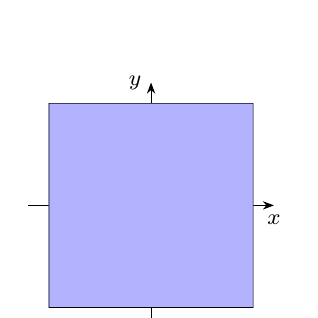
\begin{tikzpicture}[scale=1.3, baseline=(X.base)]
  \def\scale{1.3}
  \node at (0,-1) (X) {};

  \drawaxes{-1}{-1}{1}{1}
  \clip (-1,-1) rectangle (1,1);

  \draw[integration domain] (1,1) |- (-1,-1) |- cycle;
\end{tikzpicture}
&
\begin{tikzpicture}[scale=1.3, baseline=(X.base)]
  \def\scale{1.3}
  \node at (0,-1) (X) {};

  \drawaxes{-1}{-1}{1}{1}
  \clip (-1,-1) rectangle (1,1);

  \draw[integration domain]
    plot[parametric, domain=-1:1, samples=100] function {t, 0.5*t**2+0.5}
    -- plot[parametric, domain=1:-1, samples=100] function {0.5*t**2+0.5, t}
    -- plot[parametric, domain=1:-1, samples=100] function {t, -0.5*t**2-0.5}
    -- plot[parametric, domain=-1:1, samples=100] function {-0.5*t**2-0.5, t};
\end{tikzpicture}
&
\begin{tikzpicture}[scale=1.3, baseline=(X.base)]
  \def\scale{1.3}
  \node at (0,-1) (X) {};

  \drawaxes{-1}{-1}{1}{1}
  \clip (-1,-1) rectangle (1,1);

  \draw[integration domain]
    plot[parametric, domain=-1:1, samples=100] function {t, 0.5*t**2+0.5}
    -- (1,-1)
    -- plot[parametric, domain=1:-1, samples=100] function {t, -0.5*t**2-0.5}
    -- (-1,1);
\end{tikzpicture}
&
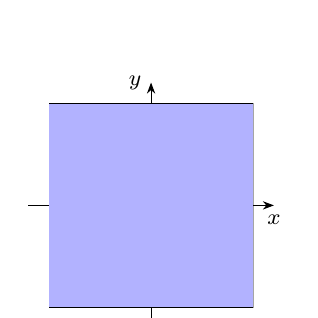
\begin{tikzpicture}[scale=1.3, baseline=(X.base)]
  \def\scale{1.3}
  \node at (0,-1) (X) {};

  \drawaxes{-1}{-1}{1}{1}
  \clip (-1,-1) rectangle (1,1);

  \draw[integration domain]
    (-1,1) -- (1,1)
    -- plot[parametric, domain=1:-1, samples=100] function {0.5*t**2+0.5, t}
    -- (1,-1) -- (-1,-1)
    -- plot[parametric, domain=-1:1, samples=100] function {-0.5*t**2-0.5, t};
\end{tikzpicture}
\\
(a) & (b) & (c) & (d)
\end{figuretable}
\end{center}
\end{solution}

\begin{question}
\SetQuestionProperties{source = {Ex. 1--2; MW, III.17.2}}
Sketch each of the following domains and determine whether it is of type 1, type 2, both or neither.
\begin{tasks}(2)
\task
$(x,y)$ such that $0 \leq y \leq 3x$, $0 \leq x \leq 1$.
\task
$(x,y)$ such that $2y^2-1 \leq x \leq y^2$, $|y| \leq 1$.
\task
$(x,y)$ such that $y^2 \leq x \leq y$, $0 \leq y \leq 1$.
\task
$(x,y)$ such that $1 - x^2 \leq 2y$, $x^2+y^2 \leq 1$.
\task
$(x,y)$ such that $x^2 + y^2 \leq 1$.
\task
$(x,y)$ such that $\displaystyle \frac 12 \leq x^2 + y^2 \leq 1$.
\end{tasks}
\end{question}

\begin{solution}
The domains can be seen in the figures below.
% \begin{center}
% \begin{figuretable}{3}
% \begin{tikzpicture}[scale=1.25, baseline=0]
%   \def\scale{1.25}

%   \drawxlabels{1/1}
%   \drawylabels{3/3}
%   \drawaxes{0}{0}{3}{3}

%   \draw[dashed] (0,3) -- (1,3);

%   \draw[integration domain] (0,0) -- (1,0) -- (1,3) -- (0,0);
%   \node at (0.66,1) {$D$};
% \end{tikzpicture}
% &
% \begin{tikzpicture}[scale=1.25, baseline=(X.base)]
%   \def\scale{1.25}
%   \node at (0,-1.5) (X) {};

%   \drawaxes{-1.5}{-1.5}{1.5}{1.5}

%   \node[above left] at (-.5,.5) {$x=2y^2-1$};
%   \node[below right] at (.5,.7) {$x=y^2$};

%   \clip (-1.5,-1.5) rectangle (1.5,1.5);

%   \draw[dashed] (0,1) -- (1,1)
%                 (0,-1) -- (1,-1);

%   \fill[integration domain]
%     plot[parametric, domain=-1:1, samples=100] function {2*t**2-1, -t}
%     --plot[parametric, domain=-1:1, samples=100] function {t**2, t};

%   \draw plot[parametric, domain=-1.5:1.5, samples=100] function {2*t**2-1, t};
%   \draw plot[parametric, domain=-1.5:1.5, samples=100] function {t**2, t};

%   \node at (-0.5,0) {$D$};

%   \drawylabels[nofill]{-1/-1, 1/1}
% \end{tikzpicture}
% &
% \begin{tikzpicture}[scale=2.5, baseline=(X.base)]
%   \def\scale{2.5}
%   \node at (0,-0.25) (X) {};

%   \drawaxes{-0.25}{-0.25}{1.25}{1.25}
%   \drawxlabels{1/1}
%   \drawylabels{1/1}

%   \draw[dashed] (1,0) -- (1,1) -- (0,1);

%   \clip (-0.25,-0.25) rectangle (1.25,1.25);

%   \fill[integration domain] (0,0) -- (1,1) 
%     --plot[domain=1:0, samples=100] function {sqrt(x)};
%   \draw (-0.25,-0.25) -- (1.25,1.25);
%   \draw plot[parametric, domain=-0.25:1.25, samples=100] function {t**2, t};

%   \node[below right] at (0.25,0.25) {$x=y$};
%   \node[above left] at (0.5,0.707) {$x=y^2$};
%   \node at (0.375,0.5) {$D$};
% \end{tikzpicture}
% \\
% (a) & (b) & (c)
% \end{figuretable}
% \end{center}

\begin{center}
\begin{figuretable}{3}
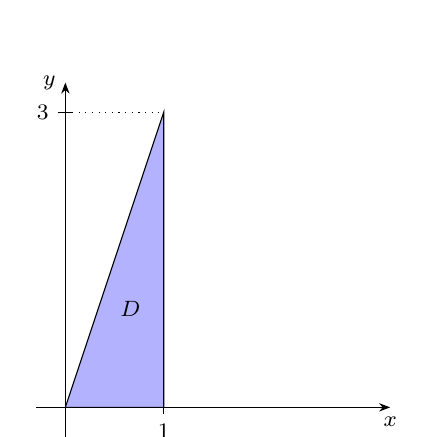
\begin{tikzpicture}[scale=1.25, baseline=0]
  \def\scale{1.25}

  \drawxlabels{1/1}
  \drawylabels{3/3}
  \drawaxes{0}{0}{3}{3}

  \draw[dotted] (0,3) -- (1,3);

  \draw[integration domain] (0,0) -- (1,0) -- (1,3) -- (0,0);
  \node at (0.66,1) {$D$};
\end{tikzpicture}
&
\begin{tikzpicture}[scale=1.25, baseline=(X.base)]
  \def\scale{1.25}
  \node at (0,-1.5) (X) {};

  \drawaxes{-1.5}{-1.5}{1.5}{1.5}

  \node[above left] at (-.5,.5) {$x=2y^2-1$};
  \node[below right] at (.5,.7) {$x=y^2$};

  \clip (-1.5,-1.5) rectangle (1.5,1.5);

  \draw[dotted] (0,1) -- (1,1)
                (0,-1) -- (1,-1);

  \draw[integration domain]
    plot[parametric, domain=-1:1, samples=100] function {2*t**2-1, -t}
    --plot[parametric, domain=-1:1, samples=100] function {t**2, t};

  \draw[dashed]
     plot[parametric, domain=1:1.5, samples=100] function {2*t**2-1, t}
     plot[parametric, domain=-1.5:-1, samples=100] function {2*t**2-1, t};
  \draw[dashed]
    plot[parametric, domain=1:1.5, samples=100] function {t**2, t}
    plot[parametric, domain=-1.5:-1, samples=100] function {t**2, t};

  \node at (-0.5,0) {$D$};

  \drawylabels[nofill]{-1/-1, 1/1}
\end{tikzpicture}
&
\begin{tikzpicture}[scale=2.5, baseline=(X.base)]
  \def\scale{2.5}
  \node at (0,-0.25) (X) {};

  \drawaxes{-0.25}{-0.25}{1.25}{1.25}
  \drawxlabels{1/1}
  \drawylabels{1/1}

  \draw[dotted] (1,0) -- (1,1) -- (0,1);

  \clip (-0.25,-0.25) rectangle (1.25,1.25);

  \draw[integration domain] (0,0) -- (1,1) 
    --plot[domain=1:0, samples=100] function {sqrt(x)};
  \draw[dashed] (-0.25,-0.25) -- (0,0)
                (1,1) -- (1.25,1.25);
  \draw[dashed]
    plot[parametric, domain=-0.25:0, samples=100] function {t**2, t}
    plot[parametric, domain=1:1.25, samples=100] function {t**2, t};

  \node[below right] at (0.5,0.5) {$x=y$};
  \node[above left] at (0.5,0.707) {$x=y^2$};
  \node at (0.375,0.5) {$D$};
\end{tikzpicture}
\\
(a) & (b) & (c)
\end{figuretable}
\end{center}

\begin{enumerate}
\item
The domain is a triangle with vertices $(0,0)$, $(1,0)$ and $(1,3)$. It is a domain of both types.
\item
This domain can be written as
\[
D = \left\{ (x,y) \,:\, -1 \leq y \leq 1,\, 2y^2 - 1 \leq x \leq y^2 \right\}\,.
\]
It is a type 2 domain, but not a type 1 domain.
\item
This domain can be written as
\begin{align*}
D &= \left\{ (x,y) \,:\, 0 \leq y \leq 1\,,\; y^2 \leq x \leq y \right\}
= \left\{ (x,y) \,:\, 0 \leq x \leq 1\,,\; x \leq y \leq \sqrt{x} \right\}\,,
\end{align*}
and hence it is a domain of both types.
\item
The domain can be written as
\[
D = \left\{ (x,y) \,:\, -1 \leq x \leq 1,\, \frac 12\left(1-x^2\right) \leq y \leq \sqrt{1-x^2} \right\}\,.
\]
It is a type 1 domain, but not a type 2 domain.
\item
The domain can be written as
\begin{align*}
D &= \left\{ (x,y) \,:\, -1 \leq y \leq 1\,,\; -\sqrt{1-y^4} \leq x \leq \sqrt{1-y^4} \right\} \\
&= \left\{ (x,y) \,:\, -1 \leq x \leq 1\,,\; -\sqrt{1-x^4} \leq y \leq \sqrt{1-x^4} \right\}\,,
\end{align*}
and it is a domain of both types.
\item
This domain is neither of type 1 nor of type 2.
\end{enumerate}

\begin{center}
\begin{figuretable}{3}
\begin{tikzpicture}[scale=1.875, baseline=(X.base)]
  \def\scale{1.875}
  \node at (0,-1) (X) {};

  \drawaxes{-1}{-1}{1}{1}

  \draw[integration domain] 
    plot[domain=-1:1, samples=100] function {0.5-0.5*x**2}
    --(1,0) arc[start angle=0, end angle=180, radius=1];

  \draw[dashed]
    (-1,0) arc[radius=1, start angle=180, end angle=360];
%  \draw plot[domain=-1:1, samples=100] function {0.5-0.5*x**2};

  \node at (0,0.75) {$D$};

  \drawxlabels[fill]{-1/-1, 1/1}
  \drawylabels[nofill]{1/1}
  \drawylabels[fill]{-1/-1}
\end{tikzpicture}
&
\begin{tikzpicture}[scale=1.875, baseline=(X.base)]
  \def\scale{1.875}
  \node at (0,-1) (X) {};

  \draw[integration domain, samples=100, smooth]
    plot[parametric, domain=0:3.1416/2] 
      function {cos(t), sin(t)}
    --plot[parametric, domain=3.1416/2:3.1416] 
      function {-(abs(cos(t))), sin(t)}
    --plot[parametric, domain=3.1416:3.1416*1.5] 
      function {-abs(cos(t)), -abs(sin(t))}
    --plot[parametric, domain=3.1416*1.5:3.1416*2] 
      function {cos(t), -abs(sin(t))}
    --(1,0) ;

  % Coordinate axes
  \drawaxes{-1}{-1}{1}{1}
  \drawxlabels[nofill]{-1/-1, 1/1}
  \drawylabels[nofill]{-1/-1, 1/1}

  % Label
  \node at (0.4,0.4) {$D$};
\end{tikzpicture}
&
\begin{tikzpicture}[scale=1.875, baseline=(X.base)]
  \def\scale{1.875}
  \node at (-1,-1) (X) {};

  \def\r{0.707106} % sqrt(2)/2

  % Draw both curves at the same time and use even odd rule to plot inside
  \draw[integration domain, samples=100, smooth, even odd rule]
    plot[parametric, domain=0:3.1416/2] 
      function {cos(t), sin(t)}
    --plot[parametric, domain=3.1416/2:3.1416] 
      function {-(abs(cos(t))), sin(t)}
    --plot[parametric, domain=3.1416:3.1416*1.5] 
      function {-abs(cos(t)), -abs(sin(t))}
    --plot[parametric, domain=3.1416*1.5:3.1416*2] 
      function {cos(t), -abs(sin(t))}
    --(1,0)
    plot[parametric, domain=0:3.1416/2] 
      function {\r*cos(t), \r*sin(t)}
    --plot[parametric, domain=3.1416/2:3.1416] 
      function {-\r*(abs(cos(t))), \r*sin(t)}
    --plot[parametric, domain=3.1416:3.1416*1.5] 
      function {-\r*abs(cos(t)), -\r*abs(sin(t))}
    --plot[parametric, domain=3.1416*1.5:3.1416*2] 
      function {\r*cos(t), -\r*abs(sin(t))}
    --(\r,0) ;

  % Coordinate axes
  \drawaxes{-1}{-1}{1}{1}
  \drawxlabels[nofill]{-1/-1, \r/\textstyle{\frac{\sqrt{2}}{2}}, 1/1}
  \drawylabels[nofill]{-1/-1, 1/1}

  % Label
  \node at (0.4,0.75) {$D$};
\end{tikzpicture}
\\
(d) & (e) & (f)
\end{figuretable}
\end{center}
\end{solution}

\begin{question}
\SetQuestionProperties{source = {Ex. 5; Guichard, 15.1}}
Evaluate the following iterated integrals.
\begin{tasks}(2)
\task
$\int_0^1 \int_0^y xy \ud x \ud y$
\task
$\int_1^4 \int_1^{\sqrt{x}} y^2 \ud y \ud x$.
\task
$\int_1^2 \int_{y^2/2}^{\sqrt y} 1 \ud x \ud y$
\task
$\int_1^2 \int_1^x \frac{x^2}{y^2} \ud y \ud x$
\task
$\int_0^1 \int_0^x \frac{y}{e^x} \ud y \ud x$
\task
$\int_0^{\sqrt{\pi}/2} \int_0^{x^2} x \cos y \ud y \ud x$
\end{tasks}
\end{question}

\begin{solution}
\begin{enumerate}
\item
\begin{alignenum}
\int_0^1 \int_0^y xy \ud x \ud y
= \int_0^1 \frac 12 x^2 y \bigg|_{x=0}^y \ud y
= \frac 12 \int_0^1 y^3 \ud y
= \frac 18\,.
\end{alignenum}
\item
\begin{alignenum}  
\int_1^4 \int_1^{\sqrt{x}} y^2 \ud y \ud x
&= \int_1^4 \frac 13 y^3 \bigg|_{y=1}^{\sqrt{x}} \ud x
= \int_1^4 \frac 13 x^{3/2} - \frac 13 \ud x 
= \frac 2{15} x^{5/2} - \frac 13 x \bigg|_{x=1}^4
%= \frac{64}{15} - \frac 4 3 - \frac 2{15} + \frac 13
= \frac{47}{15}\,.
\end{alignenum}
\item
\begin{alignenum}
\int_1^2 \int_{y^2/2}^{\sqrt y} 1 \ud x \ud y
= \int_1^2 \sqrt{y} - \frac 12 y^2 \ud y
= \frac 23 y^{3/2} - \frac 16 y^3 \bigg|_{y=1}^2
= \frac{4}{3}\sqrt{2} - \frac{11}{6}\,.
\end{alignenum}
\item
\begin{alignenum}
\int_1^2 \int_1^x \frac{x^2}{y^2} \ud y \ud x
= \int_1^2 -\frac{x^2}{y} \bigg|_{y=1}^x \ud x
= \int_1^2 -x + x^2 \ud x 
= -\frac 12 x^2 + \frac 13 x^3\bigg|_{x=1}^2
= \frac{5}{6}\,.
\end{alignenum}
\item
\begin{alignenum}
\int_0^1 \int_0^x \frac{y}{e^x} \ud y \ud x
&= \int_0^1 \frac 12 \frac{y^2}{e^x} \bigg|_{y=0}^x \ud x
= \frac 12 \int_0^1 x^2 e^{-x} \ud x
= -\frac 12 x^2 e^{-x}\bigg|_{x=0}^1 + \int_0^1 x e^{-x} \ud x \\
&= -\frac 12 e^{-1} - x e^{-x} \bigg|_{x=0}^1 + \int_0^1 e^{-x} \ud x
= -\frac 32 e^{-x} - e^{-x}|_{x=0}^1 = 1-\frac 52 e^{-x}\,.
\end{alignenum}
\item
\begin{alignenum}
\int_0^{\sqrt{\pi}/2} \int_0^{x^2} x \cos y \ud y \ud x
%= \int_0^{\sqrt{\pi}/2} x \sin y \bigg|_{y=0}^{x^2} \ud x
= \int_0^{\sqrt{\pi}/2} x \sin\left(x^2\right) \ud x
= -\frac 12 \cos \left(x^2\right) \bigg|_{x=0}^{\sqrt{\pi}/2} = \frac 12 - \frac{\sqrt 2}4\,.
\end{alignenum}
\end{enumerate}
\end{solution}

\begin{question}
\SetQuestionProperties{source = {Ex. 9--11; Thomas 12th, 15.2}}
Write an iterated integral $\iint_D f(x,y) \ud x \ud y$ over the described region, both as a type 1 domain and as a type 2 domain.
\begin{center}
\begin{figuretable}{3}
\begin{tikzpicture}[scale=1.875, baseline=(X.base)]
  \def\scale{1.875}
  \node at (0,-0.5) (X) {};

  \drawaxes{-0.5}{-0.5}{1.5}{1.5}
  \clip (-.5,-.5) rectangle (1.5,1.5);

  \draw plot[parametric, domain=-0.5:1.5, samples=100] function {t, t**3};
  \draw (-.5,1) -- (1.5,1);

  \draw[integration domain]
    plot[parametric, domain=0:1, samples=100] function {t, t**3}
    -- (0,1) -- (0,0);

  \node[below right] at (1,1) {$y=8$};
  \node[left] at (1.1, {1.1^3}) {$y=x^3$};

  \node at (0.4,0.6) {$D$};
\end{tikzpicture}
&
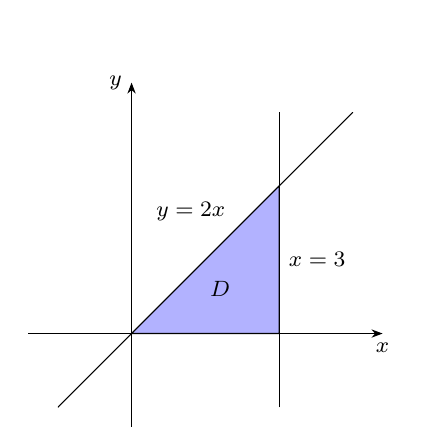
\begin{tikzpicture}[scale=1.875, baseline=(X.base)]
  \def\scale{1.875}
  \node at (0,-0.5) (X) {};

  \drawaxes{-0.5}{-0.5}{1.5}{1.5}
  \clip (-.5,-.5) rectangle (1.5,1.5);

  \draw (-.5,-.5) -- (1.5,1.5);
  \draw (1,-.5) -- (1,1.5);

  \draw[integration domain]
    (0,0) -- (1,0) -- (1,1) -- cycle;

  \node[right] at (1,.5) {$x=3$};
  \node[above left] at (.7,.7) {$y=2x$};

  \node at (0.6,0.3) {$D$};
\end{tikzpicture}
&
\begin{tikzpicture}[scale=1.875, baseline=(X.base)]
  \def\scale{1.875}
  \node at (0,-0.5) (X) {};

  \drawaxes{-0.5}{-0.5}{1.5}{1.5}
  \clip (-.5,-.5) rectangle (1.5,1.5);

  \draw plot[parametric, domain=-0.5:1.5, samples=100] function {t, t**2};
  \draw (-.5,-.5) -- (1.5,1.5);

  \draw[integration domain]
    plot[parametric, domain=0:1, samples=100] function {t, t**2}
    -- (0,0);

  \node[left] at (.8,.8) {$y=3x$};
  \node[right] at (0.7, 0.49) {$y=x^2$};

  \node at (0.5,0.375) {$D$};
\end{tikzpicture}
\\
(a) & (b) & (c)
\end{figuretable}
\end{center}
\end{question}

\begin{solution}
\begin{enumerate}
\item
The functions $y=x^3$ and $y=8$ intersect in the point $(2,8)$ and the inverse of $y=x^3$ is $x=\sqrt[3]{y}$. Thus
\[
\iint_D f(x,y) \ud x \ud y
= \int_0^2 \int_{x^3}^8 f(x,y) \ud y \ud x
= \int_0^8 \int_0^{\sqrt[3]{y}} f(x,y) \ud x \ud y\,.
\]
\item
The lines $y=2x$ and $x=3$ intersect in the point $(3,6)$ and the iverse of $y=2x$ is $x=\frac y2$. Thus
\[
\iint_D f(x,y) \ud x \ud y
= \int_0^3 \int_0^{2x} f(x,y) \ud y \ud x
= \int_0^6 \int_{y/2}^3 f(x,y) \ud x \ud y\,.
\]
\item
The functions $y=3x$ and $y=x^2$ intersect in the two points $(0,0)$ and $(3,9)$. The inverse of $y=3x$ is $x=\frac y3$ and the inverse of $y=x^2$ is $x=\sqrt y$. Thus
\[
\iint_D f(x,y) \ud x \ud y
= \int_0^3 \int_{x^2}^{3x} f(x,y) \ud y \ud x
= \int_0^9 \int_{y/3}^{\sqrt y} f(x,y) \ud x \ud y\,.
\]
\end{enumerate}
\end{solution}

\begin{question}
\SetQuestionProperties{source = {Ex. 21, 22; MW, III.17.2 and Ex. 13, 16, 17; Hartman, 13.2}}
Evaluate the following integrals
\begin{tasks}(1)
\task
$\iint_D 3-y \ud x \ud y$; $D$ is the domain between the parabolas $y^2=2x$ and $x^2=2y$.
\task
$\iint_D x^2-y^2 \ud x \ud y$; $D$ is the rectangle with vertices $(-1,-1)$, $(1,-1)$, $(1,1)$, $(-1,1)$.
\task
$\iint_D x^3y - x \ud x \ud y$; $D$ is the half of the circle $x^2 + y^2 \leq 9$ in the first and second quadrants.
\task
$\iint_D x-y \ud x \ud y$; $D$ is the triangle with vertices $(0,0)$, $(1,0)$ and $(2,2)$.
\task
$\iint_D y \cos x \ud x \ud y$; $D$ is the triangle defined by $0 \leq x \leq \pi$ and $0 \leq y \leq x$.
\task
\difficulty{*}
$\iint_D e^y \ud x \ud y$; $D$ is the domain between $y=\ln x$ and $y = \frac{1}{e-1}(x-1)$.
\end{tasks}
\end{question}

\begin{solution}
\begin{center}
\begin{figuretable}{3}
\begin{tikzpicture}[scale=1.25, baseline=(X.base)]
  \def\scale{1.25}
  \node at (0,-.5) (X) {};

  \drawaxes{-.5}{-.5}{2.5}{2.5}
  \clip (-.5,-.5) rectangle (2.5,2.5);

  \draw[dotted] (0,2) -- (2,2) -- (2,0);

  \draw[integration domain] 
    plot[parametric, domain=0:2, samples=100] function {t, sqrt(2*t)}
    -- plot[parametric, domain=2:0, samples=100] function {t, t**2/2};

  \draw[dashed]
    plot[parametric, domain=-0.5:0, samples=100] function {t, t**2/2}
    plot[parametric, domain=2:2.5, samples=100] function {t, t**2/2};
  \draw[dashed]
    plot[parametric, domain=-0.5:0, samples=100] function {t**2/2, t}
    plot[parametric, domain=2:2.5, samples=100] function {t**2/2, t};

  \node[left] at (1.2,{sqrt{2*1.2}}) {$x=y^2/2$};
  \node[right] at (.75,{.7^2/2}) {$x=\sqrt{2y}$};
  \node at (1,1) {$D$};

  \drawxlabels[fill]{2/2}
  \drawylabels[fill]{2/2}
\end{tikzpicture}
&
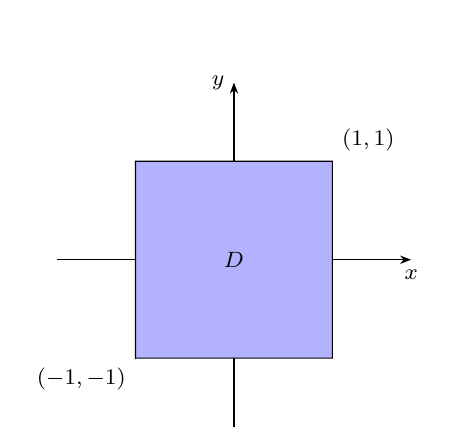
\begin{tikzpicture}[scale=1.25, baseline=(X.base)]
  \def\scale{1.25}
  \node at (0,-1.5) (X) {};

  \drawaxes{-1.5}{-1.5}{1.5}{1.5}

  \draw[integration domain] (-1,-1) -| (1,1) -| cycle;

  \node[above right] at (1,1) {$(1,1)$};
  \node[below left] at (-1,-1) {$(-1,-1)$};
  
  \node at (0,0) {$D$};
\end{tikzpicture}
&
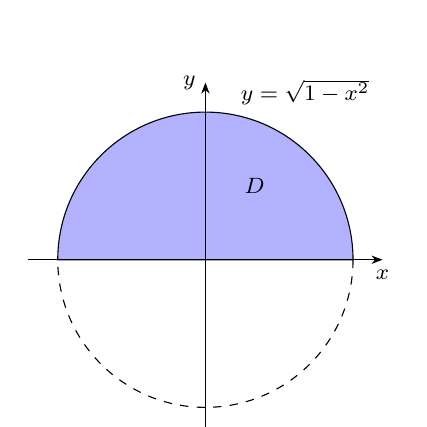
\begin{tikzpicture}[scale=0.625, baseline=(X.base)]
  \def\scale{0.625}
  \node at (-3,-3) (X) {};

  \draw[integration domain]
    (3,0) arc[radius=3, start angle=0, end angle=180] -- cycle;

  \draw[dashed]
    (3,0) arc[radius=3, start angle=0, end angle=-180];

  % Coordinate axes
  \drawaxes{-3}{-3}{3}{3}
  % \drawxlabels[fill]{-3/-3,3/3}
  % \drawylabels[nofill]{-3/-3,3/3}

  \node[above right] at (80:3) {$y=\sqrt{1-x^2}$};

  % Label
  \node at (1,1.5) {$D$};
\end{tikzpicture}
\\
(a) & (b) & (c)
\end{figuretable}
\end{center}

\begin{enumerate}
\item
The domain can be written as a type 2 domain with lower limit $x=\frac{y^2}2$ and upper limit $x = \sqrt{2y}$. Thus
\begin{align*}
\iint_D 3-y \ud x \ud y
&= \int_0^2 \int_{y^2/2}^{\sqrt{2y}} 3-y \ud x \ud y
= \int_0^2 (3-y)\left(\sqrt{2y} - \frac{y^2}{2} \right) \ud y \\
&= \int_0^2 3\sqrt 2 y^{1/2} - \sqrt 2 y^{3/2} - \frac 32 y^2 + \frac 12 y^3 \ud y \\
&= 2 \sqrt 2 y^{3/2} - \frac 25 \sqrt 2 y^{5/2} - \frac 12 y^3 + \frac 18 y^4 \bigg|_{y=0}^2
= \frac {14}5\,.
\end{align*}
\item
This is a simple iterated integral with fixed limits.
\[
\int_{-1}^1 \int_{-1}^1 x^2 - y^2 \ud x \ud y
= \int_{-1}^1 \frac 13 x^3 - xy^2 \bigg|_{x=-1}^1 \ud y
= \int_{-1}^1 \frac 23 - 2y^2 \ud y = 0\,.
\]
\item
This domain is of type 1 with lower limit $y=0$ and upper limit $y=\sqrt{3-x^2}$. Thus
\begin{align*}
\int_{-3}^3 \int_0^{\sqrt{3-x^2}} x^3 y - x \ud y \ud x
&= \int_{-3}^3 \frac 12 x^3 y^2 - xy \bigg|_{y=0}^{\sqrt{3-x^2}} \ud x
= \int_{-3}^3 \frac 12 x^3 \left(3-x^2 \right) - x \sqrt{3-x^2} \ud x \\
&= \frac 38 x^4 - \frac 1{12}x^6 + \frac 13 \left(3-x^2\right)^{3/2} \bigg|_{x=-3}^3
=0 \,.
\end{align*}
\item
The triangle is a type 2 domain and can be parametrised by
\[
D = \left\{ (x,y) \,:\, 0 \leq y \leq 2\,,\; y \leq x \leq \frac y2+1 \right\}
\]
We then have to calculate the integral
\begin{align*} 
\iint_D x-y \ud x \ud y
&= \int_0^2 \int_{y}^{y/2-2} x-y \ud x \ud y 
= \int_0^2 \frac 12 x^2 - xy \bigg|_{x=y}^{y/2-2} \ud y \\
&= \int_0^1 \frac 12 \left(\frac y2-2\right)^2 - \frac {y^2}{2} - y\left(\frac y2-2\right) + y^2 \ud y \\
&= \int_0^2 \frac{y^2}8 + y + 2 \ud y
= \frac 13 + 2 + 4 = \frac {19}3 \,.
\end{align*}
\item
This integral is best written as an integral over a type 2 domain.
\begin{align*}
\iint_D y \cos x \ud x \ud y
&= \int_0^\pi \int_y^\pi y \cos x \ud x \ud y
= \int_0^\pi y \sin x \bigg|_{x=y}^\pi \ud y
= - \int_0^\pi y \sin y \ud y \\
&= y \cos y \bigg|_{y=0}^\pi + \int_0^\pi \cos y \ud y
= -\pi\,.
\end{align*}
\item
The challenge here is to find the limits of integration. These are given by solutions of
\[
\ln x = \frac {1}{e-1} \left(x-1\right)\,.
\]
The two solutions are given by $x=1$ and $x=e$. The domain is of type 1 and therefore
\begin{align*}
\iint_D e^y \ud x \ud y
&= \int_1^e \int_{\ln x}^{(x-1)/(e-1)} e^y \ud y \ud x
= \int_1^e e^{(x-1)/(e-1)} - x \ud x \\
&= (e-1) e^{(x-1)/(e-1)} - \frac 12 x^2 \bigg|_{x=1}^e
= \frac 32 + \frac 12 e^2\,.
\end{align*}
\end{enumerate}
\begin{center}
\begin{figuretable}{3}
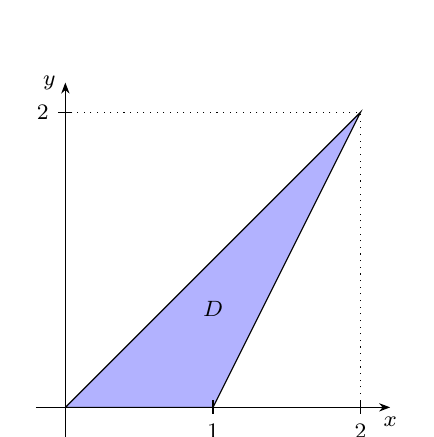
\begin{tikzpicture}[scale=1.875, baseline=(X.base)]
  \def\scale{1.875}
  \node at (0,0) (X) {};

  \drawaxes{0}{0}{2}{2}

  \draw[dotted] (2,0) -- (2,2) -- (0,2);

  \draw[integration domain]
    (0,0) -- (1,0) -- (2,2) -- cycle;

  \node at (1,0.666) {$D$};

  \drawxlabels[fill]{1/1, 2/2}
  \drawylabels[fill]{2/2}
\end{tikzpicture}
&
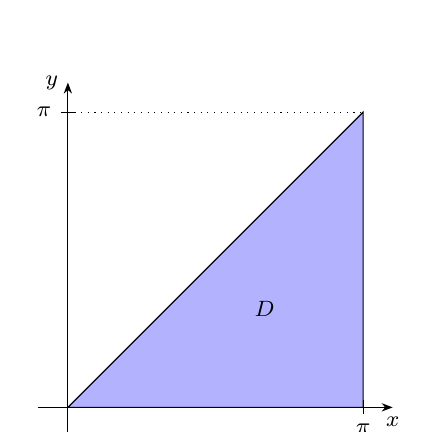
\begin{tikzpicture}[scale=3.75, baseline=(X.base)]
  \def\scale{3.75}
  \node at (0,0) (X) {};

  \drawaxes{0}{0}{1}{1}

  \draw[dotted] (0,1) -- (1,1);

  \draw[integration domain] 
    (0,0) -- (1,0) -- (1,1) -- cycle;
  
  \node at (0.666,0.333) {$D$};
  
  \drawxlabels{1/\pi};
  \drawylabels{1/\pi};
\end{tikzpicture}
&
\begin{tikzpicture}[scale=1.25, baseline=(X.base)]
  \def\scale{1.25}
  \node at (0,-1.5) (X) {};

  \drawaxes{0}{-1.5}{3}{1.5}

  \drawxlabels{1/1, 2.787/e}
  \drawylabels{1/1}

  \clip (0,-1.5) rectangle (3,1.5);

  \draw[dotted] (2.787,0) -- (2.787,1) -- (0,1);

  \draw[dashed]
    plot[parametric, domain=0.01:1, samples=100] function {t, log(t)}
    plot[parametric, domain=2.787:3, samples=100] function {t, log(t)};

  \draw[dashed] (0,{-1/(2.787-1)}) -- (1,0)
                (2.787,1) -- (3,{2/(2.787-1)});

  \draw[integration domain]
    plot[parametric, domain=1:2.787, samples=100] function {t, log(t)} -- cycle;

  \node at (1.9, 0.55) {$D$};
\end{tikzpicture}
\\
(d) & (e) & (f)
\end{figuretable}
\end{center}
\end{solution}

\begin{question}
Interpret the following iterated integrals as double integrals over a domain $D$. Sketch $D$ and change the order of integration.
\begin{tasks}(2)
\task
$\int_0^3 \int_0^{\sqrt{3}} f(x,y) \ud y \ud x$
\task
$\int_1^3 \int_0^{\ln x} f(x,y) \ud y \ud x$
\task
$\int_0^1 \int_{\arctan y}^{\pi/4} f(x,y) \ud x \ud y$
\task
$\int_{-\sqrt 2}^{\sqrt 2} \int_{y^2-1}^1 f(x,y) \ud x \ud y$
\end{tasks}
\end{question}

\begin{solution}
The domains can be seen below.
\begin{center}
\begin{figuretable}{4}
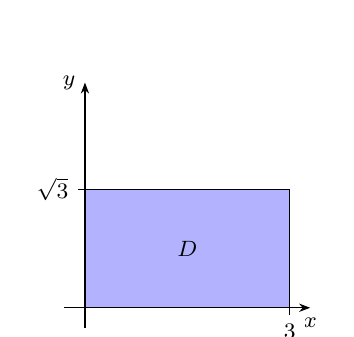
\begin{tikzpicture}[scale=1.3, baseline=(X.base)]
  \def\scale{1.3}
  \node at (0,0) (X) {};

  \drawaxes{0}{0}{2}{2}

  \draw[integration domain] (0,0) |- (2,1.155) |- cycle;

  \drawxlabels{2/3}
  \drawylabels{1.155/\sqrt{3}}

  \node at (1,.575) {$D$};
\end{tikzpicture}
&
\begin{tikzpicture}[scale=0.8666, baseline=(X.base)]
  \def\scale{0.8666}
  \node at (0,-1) (X) {};

  \drawxlabels{1/1, 3/3}
  \drawylabels{{ln(3)}/\ln 3}
  \drawaxes{0}{-1}{3}{2}

  \clip (0,-1) rectangle (3,2);

  \draw[integration domain]
    plot[parametric, domain=1:3, samples=100] function {t, log(t)}
    |- cycle;
    
  \draw[dashed]
    plot[parametric, domain=0.01:1, samples=100] function {t, log(t)};

  \draw[dotted] (0,{ln(3)}) -- (3,{ln(3)});

  \node at (2.3,0.3) {$D$};
\end{tikzpicture}
&
\begin{tikzpicture}[scale=2.6, baseline=(X.base)]
  \def\scale{2.6}
  \node at (0,0) (X) {};

  \drawylabels{1/1}
  \drawaxes{0}{0}{1}{1}
  \drawxlabels{0.785/\frac{\pi}4}


  \clip (0,0) rectangle (1,1);

  \draw[integration domain]
    plot[parametric, domain=0:1, samples=100] function {atan(t), t}
    |- cycle;

  \draw[dotted] (0,1) -- (0.785,1);

  \node at (.6,.3) {$D$};
\end{tikzpicture}
&
\begin{tikzpicture}[scale=0.8666, baseline=(X.base)]
  \def\scale{0.8666}
  \node at (0,-1.5) (X) {};

  \drawaxes{-1.5}{-1.5}{1.5}{1.5}
  \clip (-1.5,-1.5) rectangle (1.5,1.5);

  \draw[integration domain]
    plot[parametric, domain=-1.414:1.414, samples=100] function {t**2-1, t}
    -- cycle;

  \draw[dotted] (0,-1.414) -- (1,-1.414)
                (0,1.414) -- (1,1.414);

  \drawxlabels[nofill]{-1/-1,1/1}
  \drawylabels{-1.414/-\sqrt{2}, 1.414/\sqrt{2}}

  \node at (0,0) {$D$};
\end{tikzpicture}
\\
(a) & (b) & (c) & (d)
\end{figuretable}
\end{center}

\begin{enumerate}
\item
$\int_0^3 \int_0^{\sqrt{3}} f(x,y) \ud y \ud x
= \int_0^{\sqrt 3} \int_0^{3} f(x,y) \ud x \ud y$
\item
$\int_1^3 \int_0^{\ln x} f(x,y) \ud y \ud x
= \int_0^{\ln 3} \int_{e^y}^3 f(x,y) \ud x \ud y$
\item
$\int_0^1 \int_{\arctan y}^{\pi/4} f(x,y) \ud x \ud y
= \int_0^{\pi/4} \int_0^{\tan x} f(x,y) \ud y \ud x$
\item
$\int_{-\sqrt 2}^{\sqrt 2} \int_{y^2-1}^1 f(x,y) \ud x \ud y
= \int_{-1}^1 \int_{-\sqrt{x+1}}^{\sqrt{x+1}} f(x,y) \ud y \ud x$
\end{enumerate}
\end{solution}

\begin{question}
\SetQuestionProperties{source = {Ex. 17, 19, 20; MW, III.17.2}}
Sketch the region, interchange the order of integration and evaluate the integral.
\begin{tasks}(3)
\task
$\displaystyle \int_0^1 \int_x^1 xy \ud y \ud x$.
\task
$\displaystyle \int_0^1 \int_{1-y}^1 (x+y^2) \ud x \ud y$.
\task
$\displaystyle \int_1^4 \int_1^{\sqrt{x}} \left(x^2 + y^2\right) \ud y \ud x$.
\end{tasks}
\end{question}

\begin{solution} 
The regions are shown in the figures below.

\begin{center}
\begin{tabular}{ccc}
% Triangle (0,0) - (1,0) - (1,1)
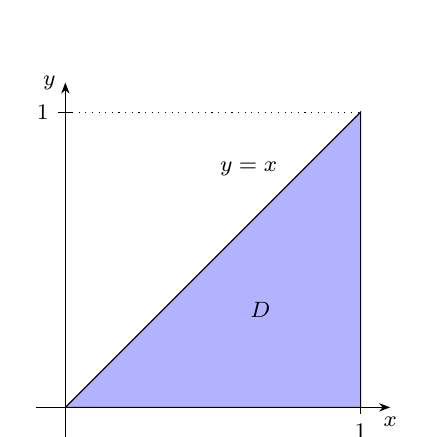
\begin{tikzpicture}[scale=3.75, baseline=0]
  \def\scale{3.75}

  \drawaxes{0}{0}{1}{1}
  \drawxlabels{1/1}
  \drawylabels{1/1}

  \draw[black,integration domain] (0,0) -- (1,0) -- (1,1) -- cycle;
  \node[above left] at (0.75, 0.75) {$y=x$};

  \draw[dotted] (0,1) -- (1,1);

  \node at (0.66,.33) {$D$};
\end{tikzpicture}
&
% Triangle (1,0) - (1,1) - (0,1)
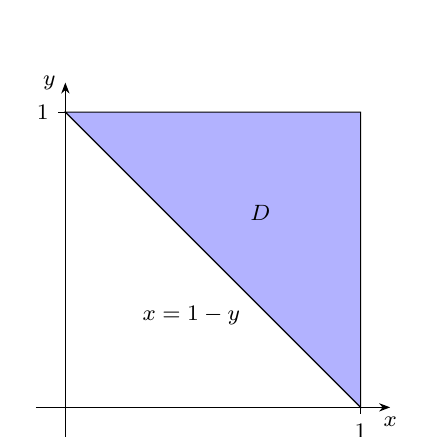
\begin{tikzpicture}[scale=3.75, baseline=0]
  \def\scale{3.75}

  \drawaxes{0}{0}{1}{1}
  \drawxlabels{1/1}
  \drawylabels{1/1}

  \draw[integration domain] (1,0) -- (1,1) -- (0,1) -- cycle;
  \node[below left, align=left] at (0.625, 0.375) {$x=1-y$};

  \node at (0.66,.66) {$D$};
\end{tikzpicture}
&
% Area between y=1, y=sqrt(x) and 1<x<4.
\begin{tikzpicture}[scale=0.9375, baseline=(BL)]
  \def\scale{0.9375}
  \coordinate (BL) at (0,-1);
  \coordinate (TR) at (4,3);

  \drawaxes{0}{-1}{4}{3}
  \drawxlabels{1/1, 4/4}
  \drawylabels{1/1, 2/2}

  \draw[dashed]
    plot[domain=0:1, samples=100, smooth] function {sqrt(x)};

  \draw[integration domain, smooth]
    plot[domain=1:4] function {sqrt(x)} |- cycle;
  \draw[dotted] (0,2) -- (4,2)
                (4,0) -- (4,1)
                (1,0) |- (0,1);

  \node[above] at (4,2) {$y=\sqrt{x}$};
  \node at (3,1.4) {$D$};
\end{tikzpicture}
\\
(a) & (b) & (c)
\end{tabular}
\end{center}

\begin{enumerate}
\item
We can write the domain as
\begin{align*}
D &= \left\{ (x,y) \,:\, 0 \leq x \leq 1\,,\; x \leq y \leq 1 \right\} \\
&= \left\{ (x,y) \,:\, 0 \leq y \leq 1\,,\; 0 \leq x \leq y \right\}\,.
\end{align*}
The integral then becomes
\[
\int_0^1 \int_x^1 xy \ud y \ud x = \int_0^1 \int_0^y xy \ud x \ud y
\]
We evaluate the latter integral
\begin{align*}
\int_0^1 \int_0^y xy \ud x \ud y
&= \int_0^1 \frac 12 x^2 y\bigg|_{x=0}^y \ud y
= \int_0^1 \frac 12 y^3 \ud y = \frac 18\,.
\end{align*}

\item
We can write the domain as
\begin{align*}
D &= \left\{ (x,y) \,:\, 0 \leq y \leq 1\,,\; 1-y \leq x \leq 1 \right\} \\
&= \left\{ (x,y) \,:\, 0 \leq x \leq 1\,,\; 1-x \leq y \leq 1 \right\}\,.
\end{align*}
The integral then becomes
\[
\int_0^1 \int_{1-y}^1 \left(x+y^2\right) \ud x \ud y = \int_0^1 \int_{1-x}^1 \left(x+y^2\right) \ud y \ud x \,.
\]
We evaluate the latter integral
\begin{align*}
\int_0^1 \int_{1-x}^1 \left(x+y^2\right) \ud y \ud x
&= \int_0^1 xy + \frac 13 y^3 \bigg|_{y=1-x}^1 \ud x
= \int_0^1 x^2 + \frac 13 - \frac 13 \left(1 - x\right)^3 \ud x \\
&= \frac 13 x^3 + \frac 13 x + \frac 1{12} \left(1-x\right)^4 \bigg|_{x=0}^1
= \frac 7{12}\,.
\end{align*}

\item
We can write the domain as
\begin{align*}
D &= \left\{ (x,y) \,:\, 1 \leq y \leq 4\,,\; 1 \leq y \leq \sqrt x \right\} \\
&= \left\{ (x,y) \,:\, 1 \leq y \leq 2\,,\; y^2 \leq x \leq 4 \right\}\,.
\end{align*}
The integral then becomes
\[
\int_1^4 \int_1^{\sqrt{x}} \left(x^2 + y^2\right) \ud y \ud x
= \int_1^2 \int_{y^2}^4 \left(x^2 + y^2 \right) \ud x \ud y\,.
\]
We evaluate the latter integral
\begin{align*}
\int_1^2 \int_{y^2}^4 \left(x^2 + y^2 \right) \ud x \ud y
&= \int_1^2 \frac 13 x^3 + y^2 x \bigg|_{x=y^2}^4 \ud y
= \int_1^2 \frac{64}3 - \frac 13 y^6 + 4y^2 - y^4 \ud y \\
&= \frac{64}{3} y - \frac 1{21}y^7 + \frac 43 y^3 - \frac 15 y^5 \bigg|_{y=1}^2
= \frac{1934}{105}\,.
\end{align*}
\end{enumerate}
\end{solution}

\begin{question}
\SetQuestionProperties{source = {MA2815 Exams, 2015}}
Evaluate the following integrals.
\begin{tasks}(2)
\task
$\int_{-1}^1 \int_1^2 \frac{x \tan^2 y}{1 + \ln y} \ud y \ud x$
\task
$\int_0^1 \int_{2x}^2 e^{-y^2} \ud y \ud x$
\task
$\int_0^2 \int_{y/2}^1 \cos\left(x^2\right) \ud x\ud y$
\task
$\int_0^1 \int_{\sqrt[3]{y}}^1 \sqrt{x^4+1} \ud x \ud y$
\task
$\int_0^2 \int_{y/2}^1 y \cos (x^3 - 1) \ud x \ud y$
\task
$\int_0^{\pi/2} \int_x^{\pi/2} \frac{\sin y}{y} \ud y \ud x$
\end{tasks}
\end{question}

\begin{solution}
\begin{center}
\begin{figuretable}{4}
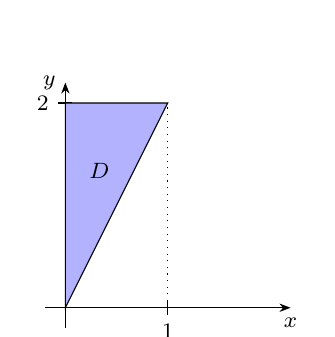
\begin{tikzpicture}[scale=1.3, baseline=(X.base)]
  \def\scale{1.3}
  \node at (0,0) (X) {};

  \drawxlabels{1/1}
  \drawylabels{2/2}

  \drawaxes{0}{0}{2}{2}

  \draw[integration domain] (0,0) -- (1,2) -| cycle;

  \draw[dotted] (1,0) -- (1,2);

  \node at (0.333, 1.333) {$D$};
\end{tikzpicture}
&
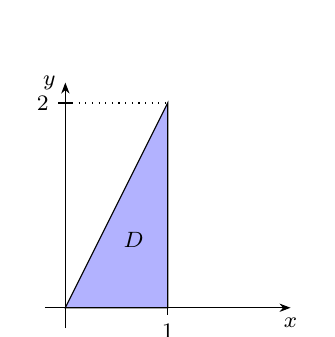
\begin{tikzpicture}[scale=1.3, baseline=(X.base)]
  \def\scale{1.3}
  \node at (0,0) (X) {};

  \drawxlabels{1/1}
  \drawylabels{2/2}

  \drawaxes{0}{0}{2}{2}

  \draw[integration domain] (0,0) -- (1,2) |- cycle;

  \draw[dotted] (0,2) -- (1,2);

  \node at (0.666, 0.666) {$D$};
\end{tikzpicture}
&
\begin{tikzpicture}[scale=2.6, baseline=(X.base)]
  \def\scale{2.6}
  \node at (0,0) (X) {};

  \drawylabels{1/1}
  \drawxlabels{1/1}
  \drawaxes{0}{0}{1}{1}

  \clip (0,0) rectangle (1,1);

  \draw[integration domain]
    plot[parametric, domain=0:1, samples=100] function {t, t**3}
    |- cycle;

  \draw[dotted] (0,1) -- (1,1);

  \node at (.8,.3) {$D$};
\end{tikzpicture}
&
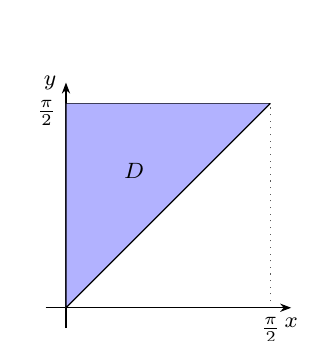
\begin{tikzpicture}[scale=2.6, baseline=(X.base)]
  \def\scale{2.6}
  \node at (0,0) (X) {};

  \node[left] at (0,.95) {$\textstyle\frac{\pi}2$};
  \node[below] at (1,0) {$\textstyle\frac{\pi}2$};
  \drawaxes{0}{0}{1}{1}
  \clip (0,0) rectangle (1,1);

  \draw[integration domain]
    (0,0) -- (1,1) -- (0,1) -- cycle;

  \draw[dotted] (1,0) -- (1,1);

  \node at (0.333,0.666) {$D$};
\end{tikzpicture}
\\
(b) & (c) \& (e) & (d) & (f)
\end{figuretable}
\end{center}
\begin{enumerate}
\item
\begin{alignenum}
\int_{-1}^1 \int_1^2 \frac{x \tan^2 y}{1 + \ln y} \ud y \ud x
= \int_1^2 \int_{-1}^1 \frac{x \tan^2 y}{1 + \ln y} \ud x \ud y
= \int_1^2 \frac 12 x^2 \cdot \frac{\tan^2 y}{1 + \ln y} \bigg|_{x=-1}^1 \ud y
= 0\,.
\end{alignenum}
\item
\begin{alignenum}
\int_0^1 \int_{2x}^2 e^{-y^2} \ud y \ud x
&= \int_0^2 \int_0^{y/2} e^{-y^2} \ud x \ud y
= \int_0^2 e^{-y^2} x \bigg|_{x=0}^{y/2} \ud y
= \int_0^2 e^{-y^2} \frac y2 \ud y \\
&= -\frac 14 e^{-y^2} \bigg|_{y=0}^2
= \frac 14 \left( 1 - e^{-4}\right)\,.
\end{alignenum}
% The region of integration can be expressed as
% \[
% \{ (x,y) \,:\, 0 \leq x \leq 1,\, 2x \leq y \leq 2 \}
% = \left\{ (x,y) \,:\, 0 \leq y \leq 2,\, 0 \leq x \leq \frac y2 \right\}\,.
% \]
% Interchanging the order of integration leads to
% \[
% I = \int_0^2 \int_0^{y/2} e^{-y^2} \ud x \ud y\,.
% \]
% The first integration is simple
% \[
% I = \int_0^2 e^{-y^2} x \bigg|_{x=0}^{y/2} \ud x = \int_0^2 e^{-y^2} \frac y2 \ud x
% \]
% Now we are also able to perform the $y$-integration
% \[
% I = -\frac 14 \int_0^2 -2y e^{-y^2} \ud y
% = -\frac 14 e^{-y^2} \bigg|_{y=0}^2 = \frac 14 \left( 1 - e^{-4}\right)\,.
% \]
\item
\begin{alignenum}
\int_0^2 \int_{y/2}^1 \cos\left(x^2\right) \ud x\ud y
&= \int_0^1 \int_0^{2x} \cos\left(x^2\right) \ud y \ud x
= \int_0^1 \cos\left( x^2 \right) y \bigg|_{y=0}^{2x} \ud x \\
&= \int_0^1 2x \cos\left(x^2\right) \ud x
= \sin\left(x^2\right) \bigg|_{x=0}^1 = \sin 1\,.
\end{alignenum}
% The region of integration can be expressed as
% \[
% \left\{ (x,y) \,:\, 0 \leq y \leq 2,\, \frac y2 \leq x \leq 1 \right\}
% = \{ (x,y) \,:\, 0 \leq x \leq 1 ,\, 0 \leq y \leq 2x \}\,.
% \]
% Interchanging the order of integration leads to
% \[
% I = \int_0^1 \int_0^{2x} \cos\left(x^2\right) \ud y \ud x\,.
% \]
% The first integration is simple
% \[
% I = \int_0^1 \cos\left( x^2 \right) y \bigg|_{y=0}^{2x} \ud x
% = \int_0^1 2x \cos\left(x^2\right) \ud x\,.
% \]
% Now we are also able to perform the $x$-integration
% \[
% I = \sin\left(x^2\right) \bigg|_{x=0}^1 = \sin 1\,.
% \]
\item
\begin{alignenum}
\int_0^1 \int_{\sqrt[3]{y}}^1 \sqrt{x^4+1} \ud x \ud y
&= \int_0^1 \int_0^{x^3} \sqrt{x^4+1} \ud y \ud x
= \int_0^1 y \sqrt{x^4 + 1} \,\bigg|_{y=0}^{x^3} \ud x \\
&= \int_0^1 x^3 \sqrt{x^4 + 1} \ud x
= \frac 16 \left(x^4 + 1\right)^{3/2} \bigg|_{x=0}^1
= \frac 16 \left(2\sqrt{2} - 1\right)\,.
\end{alignenum}
\item
\begin{alignenum}
\int_0^2 \int_{y/2}^1 y \cos \left(x^3 - 1 \right) \ud x \ud y
&= \int_0^1 \int_0^{2x} y \cos \left(x^3 - 1 \right) \ud y \ud x
= \int_0^1 \frac 12 y^2 \cos \left( x^3 - 1 \right) \bigg|_{y=0}^{2x} \ud x \\
&= \int_0^1 2x^2 \cos \left(x^3 - 1 \right) \ud x
= \frac 23 \sin \left(x^3 - 1 \right) \bigg|_{x=0}^1
= \frac 23 \sin 1\,.
\end{alignenum}
\item
\begin{alignenum}
\int_0^{\pi/2} \int_x^{\pi/2} \frac{\sin y}{y} \ud y \ud x
&= \int_0^{\pi/2} \int_0^{y} \frac{\sin y}{y} \ud x \ud y
= \int_0^{\pi/2} x \cdot \frac{\sin y}{y} \bigg|_{x=0}^y \ud y \\
&= \int_0^{\pi/2} \sin y \ud y = 1\,.
\end{alignenum}
\end{enumerate}
\end{solution}

\begin{question}
\SetQuestionProperties{difficulty = {*}}
Evaluate the iterated integral
\[
\int_0^2 \int_0^{2\sqrt{4-x^2}} \left( 4-x^2 - \frac 14 y^2\right) \ud y \ud x\,.
\]
\begin{hint*}
After performing the integration with respect to $y$, use a change of coordinates to transform the square roots from $\sqrt{4-x^2}$ to $\sqrt{1-u^2}$. Then use the trigonometric subsitution. To evaluate the resulting integral you will need to apply the half-angle formula twice.
\end{hint*}
\end{question}

\begin{solution}
We do the calculations step by step.
\begin{align*}
\int_0^2 \int_0^{2\sqrt{4-x^2}} \left( 4-x^2 - \frac 14 y^2\right) \ud y \ud x 
&= \int_0^2 8 \sqrt{4-x^2} - 2x^2 \sqrt{4-x^2} - \frac 8{12} \left(\sqrt{4-x^2}\right)^3 \ud x \\
&= \int_0^2 \frac 43 \left( \sqrt{4-x^2} \right)^3 \ud x
= \int_0^2 \frac {32}3 \left( \sqrt{1-\frac{x^2}4} \right)^3 \ud x\,.
\end{align*}
Now make the substitution $\frac x2 = u$ with $\ud x = 2 \ud u$. We obtain
\[
\int_0^2 \frac {32}3 \left( \sqrt{1-\frac{x^2}4} \right)^3 \ud x = 2 \int_0^1 \frac {32}3 \left( \sqrt{1-u^2} \right)^3 \ud u\,.
\]
Next we use the trigonometric substitution $u = \sin t$ with $\ud u = \cos t \ud t$. This leads to
\[
2 \int_0^1 \frac {32}3 \left( \sqrt{1-u^2} \right)^3 \ud u =
2 \int_0^{\pi/2} \frac {32}3 \left( \sqrt{1-\sin^2 t} \right)^3 \cos t \ud u =
\frac{64}3 \int_0^{\pi/2}  \cos^4 t \ud u\,.
\]
To evaluate this integral we use the half-angle formula twice to get
\begin{align*}
\cos^4 t &= \left( \frac{1 + \cos 2t}2 \right)^2 = \frac 14 + \frac 12 \cos 2t + \frac 14 \cos^2 2t \\
&= \frac 14 + \frac 12 \cos 2t + \frac 14 \frac{1 + \cos 4t}2 = \frac 38 + \frac 12 \cos 2t + \frac 18 \cos 4t\,.
\end{align*}
This is now easy to integrate
\[
\frac{64}3 \int_0^{\pi/2} \frac 38 + \frac 12 \cos 2t + \frac 18 \cos 4t \ud u =
\frac{64}3 \left. \left( \frac 38 t + \frac 14 \sin 2t + \frac 1{32} \sin 4t \right) \right|_{t=0}^{\pi/2} = 4 \pi\,.
\]
\end{solution}

\begin{question}
\SetQuestionProperties{difficulty = {*}}
\SetQuestionProperties{source = {Ex. 28; MW, III.17.2}}
Prove
$\int_0^x \int_0^t f(u) \ud u \ud t = \int_0^x (x-u) f(u) \ud u\,.$
\end{question}

\begin{solution}
\begin{adjustbox}{valign=T,raise=\strutheight,minipage={\linewidth}}
  \begin{wrapfigure}{r}{0.35\textwidth}
    \centering
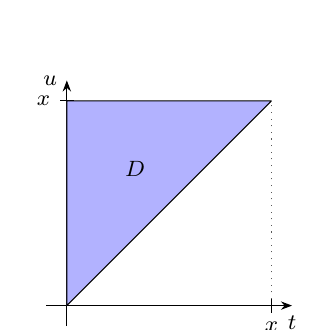
\begin{tikzpicture}[scale=2.6, baseline=(X.base)]
  \def\scale{2.6}
  \node at (0,0) (X) {};

  \drawxaxis[$t$]{0}{1}
  \drawyaxis[$u$]{0}{1}
  \drawxlabels{1/x}
  \drawylabels{1/x}
  \clip (0,0) rectangle (1,1);

  \draw[integration domain]
    (0,0) -- (1,1) -- (0,1) -- cycle;

  \draw[dotted] (1,0) -- (1,1);

  \node at (0.333,0.666) {$D$};
\end{tikzpicture}
\end{wrapfigure}
\strut{}
Treating $x$ as a constant, we change the order of integration
\begin{align*}
\int_0^x \int_0^t f(u) \ud u \ud t 
&= \int_0^x \int_u^x f(u) \ud t \ud u \\
&= \int_0^x f(u) \left( \int_0^x 1 \ud t \right) \ud u \\
&= \int_0^x (x-u) f(u) \ud u\,.
\end{align*}
\end{adjustbox}
\end{solution}


%%% Local Variables:
%%% mode: latex
%%% TeX-master: "problems"
%%% End:

\ifthenelse{\boolean{sectionnewpage}}{\newpage}{}

\section{Polar Coordinates and the Change of Coordinates}
\begin{question}
Sketch the following regions in polar coordinates.
\begin{center}
\begin{figuretable}{3}
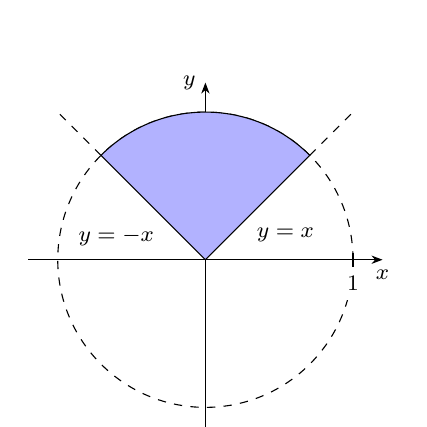
\begin{tikzpicture}[scale=1.875, baseline=(X.base)]
  \def\scale{1.875}
  \node at (0,-1) (X) {};

  \drawaxes{-1}{-1}{1}{1}

  \node[below right] at (45:.4) {$y=x$};
  \node[below left] at (135:.4) {$y=-x$};

  \draw[dashed] (0,0) circle (1);
  \draw[dashed] (45:1) -- (1,1);
  \draw[dashed] (135:1) -- (-1,1);

  \draw[integration domain] (0,0) -- (45:1)
    arc[radius=1, start angle=45, end angle=135] -- cycle;

  \drawxlabels[fill]{1/1}
\end{tikzpicture}
&
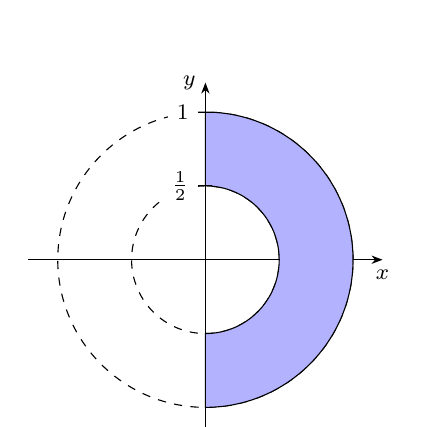
\begin{tikzpicture}[scale=1.875, baseline=(X.base)]
  \def\scale{1.875}
  \node at (0,-1) (X) {};

  \drawaxes{-1}{-1}{1}{1}

  \draw[dashed] (0,0) circle (1);
  \draw[dashed] (0,0) circle (0.5);

  \draw[integration domain] (0,0.5) -- (0,1)
    arc[radius=1, start angle=90, end angle=-90] -- (0,-.5)
    arc[radius=.5, start angle=-90, end angle=90];

  \drawylabels{.5/\frac{1}{2}, 1/1}
\end{tikzpicture}
&
\begin{tikzpicture}[scale=1.875, baseline=(X.base)]
  \def\scale{1.875}
  \node at (0,-1) (X) {};

  \drawaxes{-1}{-1}{1}{1}

  \draw[integration domain]
    plot[parametric, domain=0:2*3.1416, samples=100]
      function {sin(t)**2*cos(t), sin(t)**3};

  \node[right] at (75:1) {$r=\sin^2 \th$};
\end{tikzpicture}
\\
(a) & (b) & (c)
\end{figuretable}
\end{center}
\end{question}

\begin{solution}
In polar coordinates the domains are as follows.
\begin{center}
\begin{figuretable}{3}
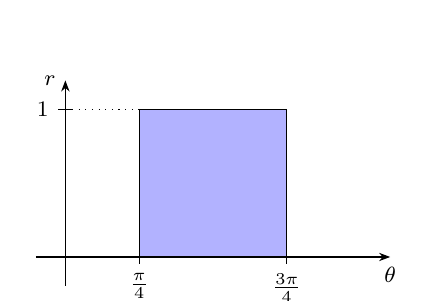
\begin{tikzpicture}[scale=1.875, baseline=(X.base)]
  \def\scale{1.875}
  \node at (0,0) (X) {};

  \drawxaxis[$\th$]{0}{2};
  \drawyaxis[$r$]{-.08}{1.08};

  \draw[integration domain] (0.5,0) -| (1.5,1) -| cycle;

  \draw[dotted] (0,1) -- (0.5,1);

  \drawylabels{1/1}
  \drawxlabels{.5/\frac{\pi}{4}, 1.5/\frac{3\pi}4}
\end{tikzpicture}
&
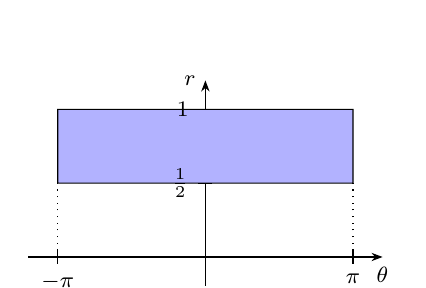
\begin{tikzpicture}[scale=1.875, baseline=(X.base)]
  \def\scale{1.875}
  \node at (0,0) (X) {};

  \drawxaxis[$\th$]{-1}{1};
  \drawyaxis[$r$]{-.08}{1.08};

  \draw[integration domain] (-1,0.5) -| (1,1) -| cycle;

  \draw[dotted] (-1,0) -- (-1,0.5)
                (1,0) -- (1,0.5);

  \drawylabels[nofill]{.5/\frac{1}{2}, 1/1}
  \drawxlabels{-1/-\pi, 1/\pi}
\end{tikzpicture}
&
\begin{tikzpicture}[scale=1.875, baseline=(X.base)]
  \def\scale{1.875}
  \node at (0,0) (X) {};

  \drawxaxis[$\th$]{-1}{1};
  \drawyaxis[$r$]{-.08}{1.08};

  \draw[integration domain]
    plot[parametric, domain=-1:1, samples=100]
      function {t, sin(t*pi)**2} -- cycle;

  %\node[above] at (0.5,1) {$r=\sin^2 \th$};

  \drawxlabels{-1/-\pi, 1/\pi}
\end{tikzpicture}
\\
(a) & (b) & (c)
\end{figuretable}
\end{center}
\end{solution}

\begin{question}
Sketch the following regions in cartesian coordinates.
\begin{center}
\begin{figuretable}{3}
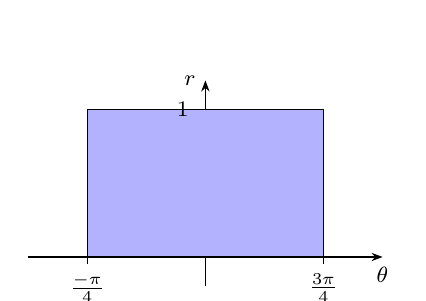
\begin{tikzpicture}[scale=1.875, baseline=(X.base)]
  \def\scale{1.875}
  \node at (0,0) (X) {};

  \drawxaxis[$\th$]{-1}{1};
  \drawyaxis[$r$]{-.08}{1.08};

  \draw[integration domain] (-.8,0) |- (.8,1) |- cycle;

  \drawxlabels{-.8/\frac{-\pi}{4}, .8/\frac{3\pi}{4}}
  \drawylabels[nofill]{1/1}
\end{tikzpicture}
&
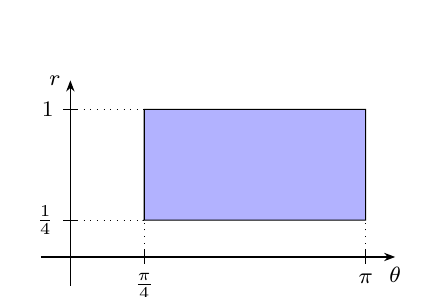
\begin{tikzpicture}[scale=1.875, baseline=(X.base)]
  \def\scale{1.875}
  \node at (0,0) (X) {};

  \drawxaxis[$\th$]{0}{2};
  \drawyaxis[$r$]{-.08}{1.08};

  \draw[integration domain] (0.5,0.25) -| (2,1) -| cycle;

  \draw[dotted] (0.5,0) -- (0.5,0.25)
                (2,0) -- (2,0.25)
                (0,0.25) -- (0.5,0.25)
                (0,1) -- (0.5,1);

  \drawylabels{.25/\frac{1}{4}, 1/1}
  \drawxlabels{.5/\frac{\pi}{4}, 2/\pi}
\end{tikzpicture}
&
\begin{tikzpicture}[scale=1.875, baseline=(X.base)]
  \def\scale{1.875}
  \node at (0,0) (X) {};

  \drawxaxis[$\th$]{-1}{1};
  \drawyaxis[$r$]{-.08}{1.08};

  \draw[integration domain]
    plot[parametric, domain=-1:1, samples=100]
      function {t, 0.5*(1+cos(pi*t))} -- cycle;

  \node[right] at (0.3,0.8) {$r=1 + \cos \th$};

  \drawxlabels{-1/-\pi, 1/\pi}
\end{tikzpicture}
\\
(a) & (b) & (c)
\end{figuretable}
\end{center}
\end{question}

\begin{solution}
In cartesian coordinates the domains are as follows.
\begin{center}
\begin{figuretable}{3}
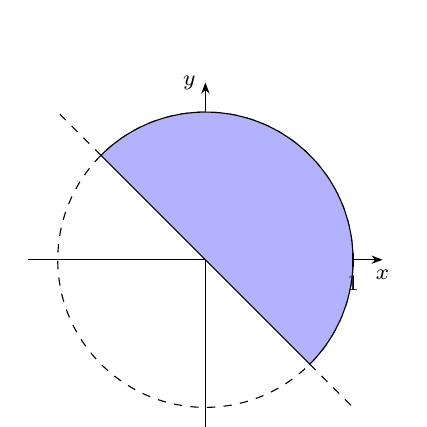
\begin{tikzpicture}[scale=1.875, baseline=(X.base)]
  \def\scale{1.875}
  \node at (0,-1) (X) {};

  \drawaxes{-1}{-1}{1}{1}

  %\node[left] at (-55:.8) {$\th=-\frac \pi 4$};
  %\node[left] at (145:.4) {$\th=\frac {3\pi}4$};

  \draw[dashed] (0,0) circle (1);
  \draw[dashed] (-45:1) -- (1,-1);
  \draw[dashed] (135:1) -- (-1,1);

  \draw[integration domain] (0,0) -- (-45:1)
    arc[radius=1, start angle=-45, end angle=135] -- cycle;

  \drawxlabels[nofill]{1/1}
\end{tikzpicture}
&
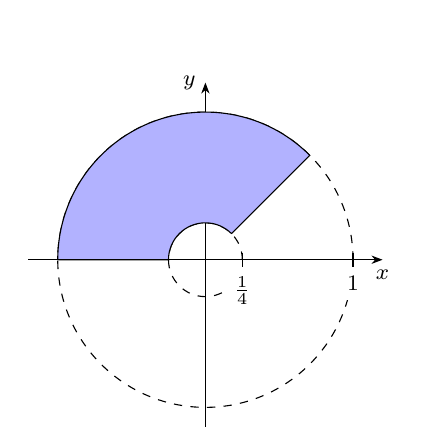
\begin{tikzpicture}[scale=1.875, baseline=(X.base)]
  \def\scale{1.875}
  \node at (0,-1) (X) {};

  \drawaxes{-1}{-1}{1}{1}

  \draw[dashed] (0,0) circle (1);
  \draw[dashed] (0,0) circle (0.25);

  \draw[integration domain] (45:0.25) -- (45:1)
    arc[radius=1, start angle=45, end angle=180] -- (-0.25,0)
    arc[radius=.25, start angle=180, end angle=45];

  \drawxlabels{.25/\frac{1}{4}, 1/1}
\end{tikzpicture}
&
\begin{tikzpicture}[scale=1.25, baseline=(X.base)]
  \def\scale{1.25}
  \node at (0,-1.5) (X) {};

  \drawaxes{-1}{-1.5}{2}{1.5};

  \draw[integration domain]
    plot[parametric, domain=0:2*pi, samples=100]
      function {(1+cos(t))*cos(t), (1+cos(t))*sin(t)};
\end{tikzpicture}
\\
(a) & (b) & (c)
\end{figuretable}
\end{center}
\end{solution}

\begin{question}
\SetQuestionProperties{source={Thomas 12th, 15.4}}
Find the limits for integrating $f(x,y)$ over the region $D$ using polar coordinates.
\begin{center}
\begin{tabu} to \linewidth {*3{X[1,c]}}
\begin{tikzpicture}[scale=1.25, baseline=(X.base)]
  \def\scale{1.25}
  \node at (0,-1.5) (X) {};

  \drawaxes{-1}{-1.5}{2}{1.5};

  \draw[dashed] (0,1) arc[radius=1, start angle=90, end angle=270];
  \draw[dashed] plot[parametric, domain=3.1416/2:3*3.1416/2, samples=100]
          function {(1+cos(t))*cos(t), (1+cos(t))*sin(t)};

  \draw[integration domain]
    plot[parametric, domain=-3.1416/2:3.1416/2, samples=100]
      function {(1+cos(t))*cos(t), (1+cos(t))*sin(t)}
    arc[radius=1, start angle=90, end angle=-90];

  \node at (1.5,0) {$D$};

  \node[above right] at (60:1.5) {$r=1+\cos \th$};
  \node[above left] at (120:1) {$r=1$};
\end{tikzpicture}
&
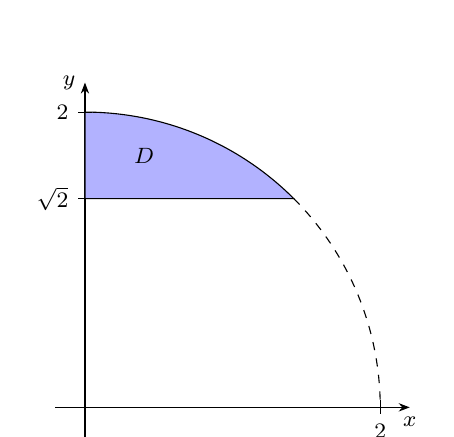
\begin{tikzpicture}[scale=1.875, baseline=(X.base)]
  \def\scale{1.875}
  \node at (0,0) (X) {};

  \drawaxes{0}{0}{2}{2}

  \draw[dashed] (45:2) arc[radius=2, start angle=45, end angle=0];
  
  \draw[integration domain] (0,2) 
    arc[radius=2, start angle=90, end angle=45] -| cycle;

  \node at (0.4,1.7) {$D$};

  \drawxlabels{2/2};
  \drawylabels{2/2, 1.414/\sqrt{2}};

\end{tikzpicture}
&
\begin{tikzpicture}[scale=1.875, baseline=(X.base)]
  \def\scale{1.875}
  \node at (0,0) (X) {};

  \drawaxes{0}{0}{2}{2}

  \draw[integration domain]
    (0,0) -- ({sqrt(3)},1) |- cycle;

  \draw[dashed] (0,1) -- ({sqrt(3)},1);

  \node at (1.2,0.4) {$D$};

  \drawxlabels{1.732/\sqrt{3}}
  \drawylabels{1/1};
\end{tikzpicture}
\\
(a) & (b) & (c)
\end{tabu}
\end{center}
\end{question}

\begin{solution}
\begin{enumerate}
\item
The integral is
\[
\int_{-\pi/2}^{\pi/2} \int_1^{1+\cos \th} f(r,\th) r \ud r \ud \th\,.
\]
\item
The line $y=\sqrt{2}$ in polar coordinates is given by
\[
r \sin \th = \sqrt{2}
\quad\Leftrightarrow\quad
r = \frac{\sqrt 2}{\sin \th}\,.
\]
It intersects the circle in the point $\left(\sqrt 2, \sqrt 2\right)$, which corresponds to $\th = \frac \pi 4$. Therefore the integral is
\[
\int_{\pi/4}^{\pi/2} \int_{\sqrt 2/\sin \th}^2 f(r,\th) r \ud r \ud \th\,.
\]
\item
The line $x=\sqrt{3}$ in polar coordinates is given by
\[
r \cos \th = \sqrt 3
\quad\Leftrightarrow\quad
r = \frac{\sqrt 3}{\cos \th}\,,
\]
and the hypothenuse of the triangle has slope $\frac{1}{\sqrt 3}$, which corresponds to $\th=\frac \pi 6$. Therefore the integral is
\[
\int_0^{\pi/6} \int_0^{\sqrt 3/\cos \th} f(r,\th) r \ud r \ud \th\,.
\]
\end{enumerate}
\end{solution}

\begin{question}
Evaluate the given integrals using polar coordinates.
\begin{tasks}(1)
\task
$\iint_D 3x-y + 4 \ud x \ud y$, where $D$ is the region enclosed by the circle $x^2 + y^2 = 1$.
\task
$\iint_D 2x - y \ud x \ud y$, where $D$ is the region in the first quadrant enclosed by the circle $x^2 + y^2 = 4$ and the lines $x=0$ and $y=x$.
\task
$\iint_D x^2 y \ud x \ud y$, where $D$ is the top half of the disk with center the origin and radius $3$.
\task
$\iint_D \ln \left(x^2 + y^2\right) \ud x \ud y$, where $D$ is the region between the circles $x^2 + y^2 = 1$ and $x^2 + y^2 = 4$.
\end{tasks}
\end{question}

\begin{solution}
The domains of integration are shown below.
\begin{center}
\begin{figuretable}{4}
\begin{tikzpicture}[scale=1.3, baseline=(X.base)]
  \def\scale{1.3}
  \node at (0,-1) (X) {};

  \drawaxes{-1}{-1}{1}{1}

  \draw[integration domain] (0,0) circle (1);

  \node at (0,0) {$D$};
  \node[right] at (60:1.05) {$r=1$};
\end{tikzpicture}
&
\begin{tikzpicture}[scale=1.3, baseline=(X.base)]
  \def\scale{1.3}
  \node at (0,0) (X) {};

  \drawaxes{0}{0}{2}{2}
  \drawxlabels[nofill]{2/2};
  \clip (0,0) rectangle (2,2);

  \draw[integration domain] (0,0) -- (2,0)
    arc[radius=2, start angle=0, end angle=45] 
    -- cycle;

  \draw[dashed] (45:2) -- (45:4);
  \draw[dashed] 
    (45:2) arc[radius=2, start angle=45, end angle=90];

  \node at (1.2,0.5) {$D$};
  \node[left] at (45:1.6) {$y=x$};
\end{tikzpicture}
&
\begin{tikzpicture}[scale=1.3, baseline=(X.base)]
  \def\scale{1.3}
  \node at (0,-1) (X) {};

  \draw[dashed]
    (1,0) arc[radius=1, start angle=0, end angle=-180];

  \drawxlabels{1/1}
  \drawaxes{-1}{-1}{1}{1}

  \draw[integration domain] 
    (1,0) arc[radius=1, start angle=0, end angle=180] -- cycle;

  \node at (0,0.4) {$D$};
\end{tikzpicture}
&
\begin{tikzpicture}[scale=1.3, baseline=(X.base)]
  \def\scale{1.3}
  \node at (0,-1) (X) {};

  \drawaxes{-1}{-1}{1}{1}

  \draw[integration domain, even odd rule]
    (0,0) circle (1)
    (0,0) circle (0.5);

  \node at (45:0.75) {$D$};
  \node[left] at (20:0.5) {$r=1$};
  \node[right] at (60:1.05) {$r=2$};
\end{tikzpicture}
\\
(a) & (b) & (c) & (d)
\end{figuretable}
\end{center}

\begin{enumerate}
\item
\begin{alignenum}
\iint_D 3x-y + 4 \ud x \ud y 
&= \int_0^1 \int_0^{2\pi} \left( 3r \cos \th - r \sin \th + 4 \right) r \ud \th \ud r \\
&= \int_0^1 3r^2 \sin \th + r^2 \cos \th + 4r\th \bigg|_{\th=0}^{2\pi} \ud r 
= \int_0^1 8\pi r \ud r = 4\pi\,.
\end{alignenum}
\item
\begin{alignenum}
\iint_D 2x-y \ud x \ud y
&= \int_0^2 \int_0^{\pi/4} \left( 2r \cos \th - r \sin \th \right) r \ud \th \ud r \\
&= \int_0^2 2r^2 \sin \th + r^2 \cos \th \bigg|_{\th=0}^{\pi/4} \ud r
= \int_0^2 \left( \frac 32 \sqrt{2} - 1\right) r^2 \ud r
= 4 \sqrt{2} - \frac 83 \,.
\end{alignenum}
\item
\begin{alignenum}
\iint_D x^2 y \ud x \ud y
&= \int_0^3 \int_0^\pi r^4 \cos^2 \th \sin \th \ud \th \ud r \\
&= \int_0^3 - \frac 13 r^4 \cos^3 \th \bigg|_{\th=0}^\pi \ud r
= \int_0^3 \frac 23 r^4 \ud r = \frac{162}{5}\,.
\end{alignenum}
\item
\begin{alignenum}
\iint_D \ln \left(x^2 + y^2 \right) \ud x \ud y
&= \int_1^2 \int_0^{2\pi} \ln\left(r^2\right) r \ud \th \ud r
= 2\pi \int_1^{\sqrt{2}} \frac 12 \ln u \ud u \\
&= \pi \left( u \ln u \bigg|_{u=1}^{\sqrt{2}} - \int_1^{\sqrt 2} 1 \ud u \right)
= \pi \left( \frac {\sqrt 2}2 \ln 2 + 1 - \sqrt 2 \right)\,.
\end{alignenum}
\end{enumerate}
\end{solution}

\begin{question}
Evaluate the given integrals.
\begin{tasks}(2)
\task
$\int_{-1}^1 \int_0^{\sqrt{1-x^2}} 1 \ud y \ud x$
\task
$\int_0^1 \int_0^{\sqrt{1-x^2}} \sqrt{x^2 + y^2} \ud y \ud x$
\task
$\int_0^{1/2} \int_{\sqrt{3}y}^{\sqrt{1-y^2}} y^2 \ud x \ud y$
\task
$\int_0^1 \int_x^{\sqrt{2-x^2}} x+2y \ud y \ud x$
\end{tasks}
\end{question}

\begin{solution}
The domains of integration are shown below.
\begin{center}
\begin{figuretable}{4}
\begin{tikzpicture}[scale=1.3, baseline=(X.base)]
  \def\scale{1.3}
  \node at (0,-1) (X) {};

  \draw[dashed]
    (1,0) arc[radius=1, start angle=0, end angle=-180];

  \drawxlabels{1/1}
  \drawaxes{-1}{-1}{1}{1}

  \draw[integration domain] 
    (1,0) arc[radius=1, start angle=0, end angle=180] -- cycle;

  \node at (0,0.4) {$D$};
\end{tikzpicture}
&
\begin{tikzpicture}[scale=1.3, baseline=(X.base)]
  \def\scale{1.3}
  \node at (0,0) (X) {};

  \draw[integration domain] (0,0) -- (2,0)
    arc[radius=2, start angle=0, end angle=90] 
    -- cycle;

  \drawaxes{0}{0}{2}{2}
  \drawxlabels[nofill]{2/1};

  \node at (45:1.33) {$D$};
\end{tikzpicture}
&
\begin{tikzpicture}[scale=1.3, baseline=(X.base)]
  \def\scale{1.3}
  \node at (0,0) (X) {};

  \drawaxes{0}{0}{2}{2}
  \drawxlabels[nofill]{2/1};
  \drawylabels{1/\textstyle\frac 12};
  \clip (0,0) rectangle (2,2);

  \draw[integration domain] (0,0) -- (2,0)
    arc[radius=2, start angle=0, end angle=30] 
    -- cycle;

  \draw[dashed] (30:2) -- (30:4);
  \draw[dashed] 
    (30:2) arc[radius=2, start angle=30, end angle=90];

  \draw[dotted] (0,1) -- (30:2);

  \node at (15:1.333) {$D$};
  \node[left] at (33:1.3) {$\textstyle \th=\frac \pi 6$};
\end{tikzpicture}
&
\begin{tikzpicture}[scale=1.3, baseline=(X.base)]
  \def\scale{1.3}
  \node at (0,0) (X) {};

  \drawaxes{0}{0}{2}{2}
  \drawxlabels[nofill]{1.414/1, 2/};
  \node[below] at (1.95,0) {$\sqrt 2$}; % Manual alignment

  \node[left] at (46:2.6) {$\textstyle\th=\frac \pi 4$};

  \clip (0,0) rectangle (2,2);

  \draw[integration domain] (0,0) -- (45:2)
    arc[radius=2, start angle=45, end angle=90] 
    -- cycle;

  \draw[dashed] (45:2) -- (45:4);
  \draw[dashed] 
    (0:2) arc[radius=2, start angle=0, end angle=45];

  \draw[dotted] (45:2)|-(0,0) -- (45:2);

  \node at (67.5:1.333) {$D$};
\end{tikzpicture}
\\
(a) & (b) & (c) & (d)
\end{figuretable}
\end{center}
We evaluate the integrals using polar coordinates.
\begin{enumerate}
\item
\begin{alignenum}
\int_{-1}^1 \int_0^{\sqrt{1-x^2}} 1 \ud y \ud x
&= \int_0^\pi \int_0^1 r \ud r \ud \th
= \int_0^\pi \frac 12 r^2 \bigg|_{r=0}^1 \ud \th = \frac \pi 2\,.
\end{alignenum}
\item
\begin{alignenum}
\int_{0}^1 \int_0^{\sqrt{1-x^2}} \sqrt{x^2 + y^2} \ud y \ud x
= \int_0^{\pi/2} \int_0^1 r^2 \ud r \ud \th
= \int_0^{\pi/2} \frac 13 r^3 \bigg|_{r=0}^1 \ud \th
= \frac \pi 6\,.
\end{alignenum}
\item
\begin{alignenum}
\int_{0}^{1/2} \int_{\sqrt 3 y}^{\sqrt{1-y^2}} y^2 \ud x \ud y
&= \int_0^{\pi/6} \int_0^1 r^3 \sin^2 \th \ud r \ud \th 
= \frac 14 \int_0^{\pi/6} \sin^2 \th \ud \th \\
&= \frac 18 \int_0^{\pi/6} 1 - \cos 2\th \ud \th
= \frac 18 \left( \th - \frac 12 \sin 2\th \right) \bigg|_{\th=0}^{\pi/6}
%= \frac \pi{48} - \frac 1{16} \sin \frac \pi 3 
= \frac \pi{48} - \frac 1{32}\,.
\end{alignenum}
\item
\begin{alignenum}
\int_0^1 \int_x^{\sqrt{2-x^2}} &x + 2y \ud y \ud x
= \int_{\pi/4}^{\pi/2} \int_0^{\sqrt 2} \left( r \cos \th + 2r \sin \th \right) 
\cdot r \ud r \ud \th \\
&= \int_{\pi/4}^{\pi/2} \frac 13 r^3 \left( \cos \th + 2 \sin \th \right)
\bigg|_{r=0}^{\sqrt 2} \ud \th
= \frac 23 \sqrt 2 \int_{\pi/4}^{\pi/2} \cos \th + 2 \sin \th \ud \th \\
&= \frac 23 \sqrt 2 \left( \sin \th - 2 \cos \th \right) \bigg|_{\th=\pi/4}^{\pi/2}
= \frac 23 \sqrt 2 \left( 1- \frac{\sqrt 2}2 + 2 \frac{\sqrt{2}}2 \right)
= \frac 23 \left(1 + \sqrt 2\right)\,.
\end{alignenum}
\end{enumerate}
\end{solution}

\begin{question}
\SetQuestionProperties{source={Ex. 27, 29, 30; Thomas 12th, 15.4}}
Find the following areas.
\begin{tasks}(1)
\task
The area enclosed by the positive $x$-axis and the spiral $r=\frac 32 \th$ with $0 \leq \th \leq 2\pi$. The area looks like a snail shell.
\task
The area enlosed by the cardioid $r = 1 + \cos \th$.
\task
The area cut from the first quadrant by the curve $r=2\sqrt{2-\sin 2\th}$.
\task
The area enclosed by one leaf of the rose $r = 12 \cos 3\th$.
\end{tasks}
\end{question}

\begin{solution}
The areas can be seen below.
\begin{center}
\begin{figuretable}{4}
\begin{tikzpicture}[scale=1.3, baseline=(X.base)]
  \def\scale{1.3}
  \node at (0,-1) (X) {};

  \drawaxes{-1}{-1}{1}{1}
 
  \clip (-1,-1) rectangle (1.1,1.1);

  \draw[integration domain] 
    plot[parametric, domain=0:2*pi, samples=100] 
      function {1.5*t*cos(t)/(3*pi), 1.5*t*sin(t)/(3*pi)}
    -- cycle;

  \draw[dashed]
    plot[parametric, domain=2*pi:2.5*pi, samples=100] 
      function {1.5*t*cos(t)/(3*pi), 1.5*t*sin(t)/(3*pi)};

  \node at (0.333,-0.33) {$D$};
  \node[above left] at (100:0.25) {$\textstyle r=\frac 32 \th$};
\end{tikzpicture}
&
\begin{tikzpicture}[scale=0.8666, baseline=(X.base)]
  \def\scale{0.8666}
  \node at (0,-1.5) (X) {};

  \drawaxes{-1}{-1.5}{2}{1.5};

  \draw[integration domain]
    plot[parametric, domain=0:2*pi, samples=100]
      function {(1+cos(t))*cos(t), (1+cos(t))*sin(t)};

  \node at (1,0) {$D$};

  \node[above right] at (80:1.3) {$r=1+\cos \th$};
\end{tikzpicture}
&

\begin{tikzpicture}[scale=0.3714, baseline=(X.base)]
  \def\scale{0.3714}
  \node at (0,-3.5) (X) {};

  \drawaxes{-3.5}{-3.5}{3.5}{3.5};

  \node[below right, fill=white] at (-3.5,-2.8) 
    {$r=2\sqrt{2-\sin 2\th}$};

  \draw[integration domain]
    plot[parametric, domain=0:2*pi, samples=100]
      function {2*sqrt(2-sin(2*t))*cos(t), 2*sqrt(2-sin(2*t))*sin(t)};

  \node at (0,0) {$D$};
\end{tikzpicture}
&
\begin{tikzpicture}[scale=1.3, baseline=(X.base)]
  \def\scale{1.3}
  \node at (0,-1) (X) {};

  \drawaxes{-1}{-1}{1}{1}

  \draw[integration domain]
    plot[parametric, domain=-pi/6:pi/6, samples=100]
      function {cos(3*t)*cos(t), cos(3*t)*sin(t)};

  \draw[dashed]
    plot[parametric, domain=pi/6:5*pi/6, samples=100]
      function {cos(3*t)*cos(t), cos(3*t)*sin(t)};

  \node at (0.6,0) {$D$};
  \node at (0.5,0.35) {$r=12 \cos 3\th$};
\end{tikzpicture}
\\
(a) & (b) & (c) & (d)
\end{figuretable}
\end{center}
We denote the area by $A$.
\begin{enumerate}
\item
\begin{alignenum}
A &= \int_0^{2\pi} \int_0^{3\th/2} r \ud r \ud \th
= \int_0^{2\pi} \frac 12 r^2 \bigg|_{r=0}^{3\th/2} \ud \th
= \int_0^{2\pi} \frac 98 \th^2 \ud \th
= 3\pi^3\,.
\end{alignenum}
\item
\begin{alignenum}
A &= \int_0^{2\pi} \int_0^{1 + \cos \th} r \ud r \ud \th
= \int_0^{2\pi} \frac 12 \left( 1 + \cos \th\right)^2 \ud \th
= \frac 12 \int_0^{2\pi} 1 + 2 \cos \th + \cos^2 \th \ud \th \\
&= \pi + \frac 14 \int_0^{2\pi} 1 + \cos 2\th \ud \th
= \frac {3\pi}2 + \frac 18 \sin 2\th \bigg|_{\th=0}^{2\pi} = \frac {3\pi}2\,.
\end{alignenum}
\item
\begin{alignenum}
A &= \int_0^{\pi 4} \int_0^{2\sqrt{2-\sin 2\th}} r \ud r \ud \th 
= \int_0^{\pi 4} \frac 12 \cdot 4 
\left( 2 - \sin 2\th \right) \ud \th
= \pi - \int_0^{\pi/4} 2 \sin 2 \th \ud \th \\
&= \pi + \cos 2 \th \bigg|_{\th=0}^{\pi/4}
= \pi - 1\,.
\end{alignenum}
\item
\begin{alignenum}
A &= \int_{-\pi/6}^{\pi/6} \int_0^{12 \cos 3\th} r \ud r \ud \th
= \int_{-\pi/6}^{\pi/6} \frac 12 r^2 \bigg|_{\th=0}^{12 \cos 3 \th} \ud \th
= 72 \int_{-\pi/6}^{\pi/6} \cos^2 3\th \ud \th \\
&= 36 \int_{-\pi/6}^{\pi/6} 1 - \cos 6 \th \ud \th
= 12\pi - 6 \sin 6\th \bigg|_{\th=-\pi/6}^{\pi/6} = 12 \pi\,.
\end{alignenum}
\end{enumerate}
\end{solution}

\begin{question}
\SetQuestionProperties{difficulty={*}}
Evaluate the following integrals using polar coordinates.
\begin{tasks}(1)
\task
$\iint_D \arctan \frac y x \ud x \ud y$;
$D = \{ (x,y)\,:\, 1 \leq x^2 + y^2 \leq 4,\, y \leq x \}$.
\task
$\iint_D \frac{x-y}{x+y} \ud x \ud y$; $D$ is the region enclosed by the lines $y=x$, $y=0$ and the circle $x^2 + y^2 = 1$ in the first quadrant.
\end{tasks}
\end{question}

\begin{solution}
\begin{enumerate}
\item
\begin{adjustbox}{valign=T,raise=\strutheight,minipage={\linewidth}}
  \begin{wrapfigure}{r}{0.35\textwidth}
    \centering
\begin{tikzpicture}[scale=1.875, baseline=(X.base)]
  \def\scale{1.875}
  \node at (0,-1) (X) {};

  \drawaxes{-1}{-1}{1}{1}

  \node[left] at (45:1.4) {$y=x$};

  \draw[dashed] (0,0) circle (1);
  \draw[dashed] (0,0) circle (0.5);
  \draw[dashed] (-1,-1) -- (1,1);

  \draw[integration domain] (45:0.5) -- (45:1)
    arc[radius=1, start angle=45, end angle=-90] -- (-90:0.5)
    arc[radius=.5, start angle=-90, end angle=45];

  \draw[integration domain2] (-90:0.5) -- (-90:1)
    arc[radius=1, start angle=-90, end angle=-135] -- (-135:0.5)
    arc[radius=.5, start angle=-135, end angle=-90];

  \drawylabels[fill]{.5/1, 1/2}
\end{tikzpicture}
\end{wrapfigure}
\strut{}
The line $y=x$ splits the plane into two regions. 
In polar coordinates we can describe the regions as follows: the region above the line consists of points with $\frac \pi 4 \leq \th \leq \frac {5\pi}4$ and the region below the line consists of those points with $-\frac{3\pi}{4} \leq \th \leq \frac \pi 4$. Thus the domain $D$ is a rectangle in polar coordinates,
\[
D' = \left\{ (r,\th) \,:\, 1 \leq r \leq 2,\, -\frac{3\pi}4 \leq \th \leq \frac \pi 4 \right\}\,.
\]
To rewrite the function in polar coordinates we use that
\[
\tan \th = \frac y x\,,
\]
and so 
\end{adjustbox}
\[
f(r,\th) = \arctan \tan \th\,.
\]
Before we make the simplification $\arctan \tan \th = \th$ we have to be careful that $\arctan$ chooses the right branch of $\tan$. Indeed, since by convention $\arctan$ takes values in the interval $\left[-\frac \pi 2, \frac \pi 2\right]$, we find that
\[
\arctan \tan \th = \begin{cases}
\th & \th \in \left[-\frac \pi 2, \frac \pi 4\right] \\
\th + \pi & \th \in \left[-\frac {3\pi} 4, -\frac \pi 2\right]
\end{cases}
\]
So we split domain into two parts and recombine the integrals to get
\begin{align*}
\iint_D \arctan \frac y x \ud x \ud y &= \int_{\pi/2}^{\pi/4} \int_1^2\th r \ud r \ud \th
+ \int_{-3\pi/4}^{-\pi/2} \int_1^2(\th+\pi)r \ud r \ud \th \\
&=\int_{-3\pi/4}^{\pi/4} \int_1^2\th r \ud r \ud \th
+ \pi \int_{-3\pi/4}^{-\pi/2} \int_1^2 r \ud r \ud \th
\end{align*}
Both integrals can be calculated without too much difficulty,
\begin{align*}
\int_{-3\pi/4}^{\pi/4} \int_1^2\th r \ud r \ud \th
&= \int_{-3\pi/4}^{\pi/4} \left. \frac {r^2}2 \th \right|_{r=1}^2 \ud \th
= \frac 32 \int_{-3\pi/4}^{\pi/4} \th \ud \th
= \frac 32 \left. \frac {\th^2} 2 \right|_{\th = -3\pi/4}^{\pi/4} \\
&= \frac 34 \left( \frac {\pi^2}{16} - \frac{9\pi^2}{16} \right)
= -\frac {3\pi^2}8\,,
\end{align*}
and the second one
\begin{align*}
\pi \int_{-3\pi/4}^{-\pi/2} \int_1^2 r \ud r \ud \th &= \pi \left( -\frac \pi 2 + \frac{3\pi}4 \right)
\left. \frac{r^2}2 \right|_{r=1}^2 = \frac{3\pi^2}8\,.
\end{align*}
Thus we obtain
\[
\iint_D \arctan \frac y x \ud x \ud y = 0\,.
\]

\item
\begin{adjustbox}{valign=T,raise=\strutheight,minipage={\linewidth}}
  \begin{wrapfigure}{r}{0.35\textwidth}
    \centering
\begin{tikzpicture}[scale=1.875, baseline=(X.base)]
  \def\scale{1.875}
  \node at (0,-1) (X) {};

  \drawaxes{-1}{-1}{1}{1}

  \node[left] at (45:1.4) {$y=x$};

  \draw[dashed] (0,0) circle (1);
  \draw[dashed] (45:1) -- (1,1);

  \draw[integration domain] (0,0) -- (1,0)
    arc[radius=1, start angle=0, end angle=45] -- cycle;

  \drawylabels[fill]{1/1}
\end{tikzpicture}
\end{wrapfigure}
\strut{}
In polar coordinates the integral becomes
\begin{align*}
\iint_D \frac{x-y}{x+y} \ud x \ud y
&= \int_0^{\pi/4} \int_0^1 \frac{\cos \th - \sin \th}{\cos \th + \sin \th} 
r \ud r \ud \th \\
&= \frac 12 \int_0^{\pi/4} \frac{\cos \th - \sin \th}{\cos \th + \sin \th} \ud \th\,.
\end{align*}
To continue we multiply the both parts of the fraction by $\cos \th + \sin \th$, we leads to
\begin{align*}
\iint_D \frac{x-y}{x+y} \ud x \ud y
&= \frac 12 \int_0^{\pi/4} \frac{\cos^2 \th - \sin^2 \th}{1 + 2\cos \th \sin \th} \ud \th \\
&= \frac 12 \int_0^{\pi/4} \frac{\cos 2\th}{1+\sin 2\th} \ud \th \\
&= \frac 14 \ln \left(1 + \sin 2\th\right) \bigg|_{\th=0}^{\pi/4} \\
&= \frac 14 \ln 2\,.
\end{align*}
\end{adjustbox}
\end{enumerate}
\end{solution}

\begin{question}
Using the general change of variables formula und $u=x+y$, $y=uv$, show that
\[
\int_0^1 \int_0^{1-x} e^{y/(x+y)} \ud y \ud x = \frac{e-1}2\,.
\]
\end{question}

\begin{solution}
The change of variables can be expressed as
\begin{align*}
x &= u(1-v) & u &= x+y \\
y &= uv & v &= \frac{y}{x+y}\,.
\end{align*}
The domain in $xy$-coordinates is the triangle with vertices $(0,0)$, $(1,0)$ and $(0,1)$. The side $x=0$ gets mapped to $v=1$, the side $y=0$ to $v=0$ and the side $y=1-x$ to $u=1$. Note also that the point $(0,0)$ becomes the line $u=0$ in the new coordinates. Thus the domain $D'$ in $uv$-coordinates is
\[
D' = [0,1] \x [0,1]\,.
\]
The derivative matrix is
\[
\frac{\p(x,y)}{\p(u,v)} = \begin{pmatrix}
1-v & -u \\ v & u
\end{pmatrix}\,,
\]
and its determinant is $\left| \frac{\p(x,y)}{\p(u,v)} \right| = u$. Thus the integral becomes
\[
\int_0^1 \int_0^{1-x} e^{y/(x+y)} \ud y \ud x = 
\int_0^1 \int_0^1 e^v u \ud u \ud v = \frac{e-1}{2}\,.
\]
\end{solution}

\begin{question}
Let $D$ be the region bounded by $x+y=1$, $x=0$, $y=0$. Use the general change of variables formula to show that
\[
\iint_D \cos\left(\frac{x-y}{x+y}\right) \ud x \ud y = \frac 12 \sin 1\,,
\]
and graph $D$ on an $xy$-plane and a $uv$-plane, with $u=x-y$ and $v=x+y$.
\end{question}

\begin{solution}
The change of variables can be expressed as
\begin{align*}
x &= \frac 12(v+u) & u &= x-y \\
y &= \frac 12(v-u) & v &= x+y\,.
\end{align*}
To transform the region we observe that the edge $x+y=1$ transforms to $v=1$; the edge $x=0$ becomes $v=-u$ and the edge $y=0$ becomes $v=u$. Thus we are integrating over the triangle with vertices $(-1,1)$, $(1,1)$ and $(0,0)$. This triangle can be parametrized as
\[
D' = \left\{ (u,v) \,:\, 0 \leq v \leq 1,\, -v \leq u \leq v \right\}\,.
\]
The derivative matrix is
\[
\frac{\p(x,y)}{\p(u,v)} = \begin{pmatrix}
\frac 12  & \frac 12 \\
-\frac 12 & \frac 12
\end{pmatrix}\,,
\]
and its determinant is $\left| \frac{\p(x,y)}{\p(u,v)} \right| = \frac 12$. Thus the integral becomes
\begin{align*}
\iint_D \cos\left(\frac{x-y}{x+y}\right) \ud x \ud y &= 
\int_0^1 \int_{-v}^v \cos\left(\frac uv\right) \cdot \frac 12 \ud u \ud v
= \frac 12 \int_0^1 v \sin\left(\frac uv\right) \bigg|_{u=-v}{v} \ud v \\
&= \int_0^1 v \sin 1 \ud v = \frac 12 \sin 1\,.
\end{align*}
\end{solution}

%%% Local Variables:
%%% TeX-master: "problems"
%%% End:

\ifthenelse{\boolean{sectionnewpage}}{\newpage}{}

\section{Applications of the Double Integral}
\begin{question}
Find the volume under the graph of
\[
f(x,y) = xy\sqrt{x^2 -y^2}
\]
between the planes $x=1$, $x=2$, $y=0$ and $y=1$.
\end{question}

\begin{solution}
The volume $V$ can be computed as the integral
\begin{align*}
V
&= \int_1^2 \int_0^1 xy \sqrt{x^2-y^2} \ud y \ud x
= \int_0^1 -\frac 13 x \left( x^2-y^2\right)^{3/2} \bigg|_{y=0}^1 \ud x \\
&= \frac 13 \int_1^2 x^4 - x \left(x^2-1\right)^{3/2} \ud x
= \frac 1{15} \left( x^5 - \left(x^2-1\right)^{5/2} \right) \bigg|_{x=1}^2
= 2\,.
\end{align*}
Therefore the volume is $2$.
\end{solution}

\begin{question}
Find the volume under the graph of
\[
f(x,y) = 1+\sin\left( \frac{\pi y}{2}\right) +2x
\]
on the domain enclosed by the parallelogram with the vertices $(0,0)$, $(1,2)$, $(2,0)$ and $(3,2)$.
\end{question}

\begin{solution}
The domain $D$ enclosed by the parallelogram is of type $2$ domain and can be written as
\[
D = \left\{ (x,y) \,:\, 0 \leq y \leq 2\,,\; \frac y2 \leq x \frac y2 + 2 \right\}\,.
\]
Thus the volume is given by the integral
\begin{align*}
V
&=\int_0^2 \int_{y/2}^{y/2+2} 1 + \sin \left(\frac{\pi y}2 \right) + 2x \ud x \ud y\,,
= \int_0^2 2 + 2 \sin \left( \frac{\pi y}{2} \right) + \left( \frac y2 + 2\right)^2 - \frac{y^2}4 \ud y \\
&= \int_0^2 6 + 2y + 2 \sin \left( \frac{\pi y}2 \right) \ud y
= 6y + y^2 - \frac 4\pi \cos \left(\frac {\pi y}2 \right) \bigg|_{y=0}^2
= 16 + \frac 8\pi\,.
\end{align*}
Therefore the volume is $16 + \frac 8\pi$.
\end{solution}

\begin{question}
Find the volume between the graphs of the functions 
\[
f(x,y) = 2x+1
\qquad\text{and}\qquad
g(x,y)=-x-3y-5
\]
on the region bounded by the $y$-axis and the curve $x=4-y^2$.
\end{question}

\begin{solution}
We write region $D$ as a type 1 domain,
\[
D = \left\{ (x,y) \,:\, 0 \leq x \leq 4\,,\; -\sqrt{4-x} \leq y \leq \sqrt{4-x} \right\}\,.
\]
The volume $V$ is given by the integral
\begin{align*}
V &= \iint_D 2x+1 - (-x-3y-5) \ud x \ud y
= \int_0^4 \int_{-\sqrt{4-x}}^{\sqrt{4-x}} 3x+3y+6 \ud y \ud x \\
&= \int_0^4 6(x+2) \sqrt{4-x} \ud x
= -4(x+2) \left(4-x\right)^{3/2}\bigg|_{x=0}^4 + \int_0^4 4 \left(4-x\right)^{3/2} \ud x \\
&= -64 - \frac 85 \left(4-x\right)^{5/2} \bigg|_{x=0}^4
= -\frac{64}5\,.
\end{align*}
\end{solution}

\begin{question}
Find the average value of the function
\[
f(x,y) = x \sin xy\,,
\]
over the region $D = [0,\pi] \x [0,\pi]$.
\end{question}

\begin{solution}
The region is a rectangle with area
\[
\on{area}(D) = \pi^2\,.
\]
Next we need to compute the integral
\begin{align*}
\int_0^\pi \int_0^\pi x \sin xy \ud y \ud x
&= \int_0^\pi -\cos xy \bigg|_{y=0}^\pi \ud x
= \int_0^\pi 1 - \cos \pi x \ud x
= x - \frac 1\pi \sin \pi x \bigg|_{x=0}^\pi \\
&= \pi - \frac 1\pi \sin \pi^2\,.
\end{align*}
Therefore the average value is $\frac 1\pi - \frac 1{\pi^3} \sin \pi^2$.
\end{solution}

\begin{question}
%\SetQuestionProperties{source = {Ex. 13; MW, III.17.3}}
Find the average value of the function
\[
f(x,y) = e^{x+y}
\]
on the triangle with vertices at $(0,0)$, $(0,1)$ and $(1,0)$.
\end{question}

\begin{solution}
Denote the domain of integration by $D$. We can represent it as
\[
D = \left\{ (x,y) \,:\, 0 \leq x \leq 1\,,\; 0 \leq y \leq 1-x \right\}\,.
\]
The area of the triangle is
\[
\on{area}(D) = \frac 12\,.
\]
Next we need to compute the integral
\begin{align*}
\int_0^1 \int_0^{1-x} e^{x+y} \ud y \ud x 
&= \int_0^1 e^{x+y} \bigg|_{y=0}^1 \ud x
= \int_0^1 e - e^x \ud x
= ex - e^x \bigg|_{x=0}^1 = e - e + 1 = 1\,.
\end{align*}
Hence the average value is $2$.
\end{solution}

\begin{question}
Find the average height of the hemispherical surface $z = \sqrt{c^2 - x^2 - y^2}$ above the disk $x^2 + y^2 \leq c^2$, where $c$ is a constant.
\end{question}

\begin{solution}
The area of the disk $D$ is
\[
\on{area}(D) = c^2 \pi\,.
\]
We need to compute the integral, which we do using polar coordinates,
\begin{align*}
\iint_D \sqrt{c^2 - x^2 - y^2} \ud x \ud y
&= \int_0^c \int_0^{2\pi} \sqrt{c^2 - r^2} \cdot r \ud \th \ud r
= 2\pi \int_0^c \sqrt{c^2 - r^2} \cdot r \ud r \\
&= -\frac 23 \pi \left(c^2 - r^2\right)^{3/2} \bigg|_{r=0}^c
= \frac 23 c^3 \pi\,.
\end{align*}
Therefore the average value is $\frac 2{3} c$.
\end{solution}

\begin{question}
Find the average distance from a point $(x,y)$ in the disk $x^2 + y^2 \leq c^2$ to the origin.
\end{question}

\begin{solution}
The distance of a point to the origin is given by the function
\[
d(x,y) = \sqrt{x^2 + y^2}\,.
\]
Denote the disk by $D$. To compute the average we need to evaluate the integral, for which we use polar coordinates,
\begin{align*}
\iint_D \sqrt{x^2 + y^2} \ud x \ud y
= \int_0^c \int_0^{2\pi} r \cdot r \ud \th \ud r
= 2\pi \int_0^c r^2 \ud r
= \frac 23 \pi r^3 \bigg|_{r=0}^c
= \frac 23 c^3 \pi\,.
\end{align*}
Because the area of the disk is $c^2\pi$, the average distance is $\frac 23 c$.
\end{solution}

\begin{question}
Find the center of mass of the triangular region cut from the first quadrant by the line $x+y=3$.
\end{question}

\begin{solution}
Denote the region by $D$. Its area is
\[
\on{area}(D) = \frac {3\cdot 3}{2} = \frac 92\,.
\]
Next we calculate the integral
\begin{align*}
\iint_D x \ud x \ud y 
&= \int_0^3 \int_0^{3-x} x \ud y \ud x
= \int_0^3 x(3-x) \ud x = \frac 32 x^2 - \frac 13 x^3 \bigg|_{x=0}^3
= \frac 92\,.
\end{align*}
Because the region $D$ remains unchanged when we swap $x$ and $y$ coordinates, the other integral has the same value,
\[
\iint_D y \ud x \ud y = \frac 92.
\]
Therefore the center of mass has the coordinates
\[
\bar x = 1
\quad\text{and}\quad
\bar y = 1\,.
\]
\end{solution}

\begin{question}
Find the center of mass cut from the first quadrant by the circle $x^2 + y^2 = a^2$.
\end{question}

\begin{solution}
Denoting the region by $D$ we find that its area is
\[
\on{area} (D) = \frac 14 a^2 \pi\,.
\]
Next we calculate the integral
\begin{align*}
\iint_D x \ud x \ud y
&= \int_0^a \int_0^{\sqrt{a^2-x^2}} x \ud y \ud x
= \int_0^a x \sqrt{a^2-x^2} \ud x
= -\frac 13 \left(a-x^2\right)^{3/2} \bigg|_{x=0}^a
= \frac 13 a^3\,.
\end{align*}
Because the region $D$ remains unchanged when we swap $x$ and $y$ coordinates, the other integral has the same value,
\begin{align*}
\iint_D y \ud x \ud y = \frac 13 a^3\,.
\end{align*}
Therefore the center of mass has the coordinates
\[
\bar x = \frac {4a}{3\pi}
\quad\text{and}\quad
\bar y = \frac {4a}{3\pi}\,.
\]
\end{solution}

\begin{question}
Find the centre of mass of the region between $y=0$, $y=x^2$, where $0 \leq x \leq \frac 12$.
\end{question}

\begin{solution}
First we need to find the mass $m$ of the domain. We have
\begin{align*}
m = \int_0^{1/2} \int_0^{x^2} 1 \ud y \ud x
= \int_0^{1/2} x^2 \ud x = \frac 13 x^3 \bigg|_{x=0}^{1/2} = \frac 1{24}\,.
\end{align*}
Next we calculate the integral
\begin{align*}
\int_0^{1/2} \int_0^{x^2} x \ud y \ud x = \int_0^{1/2} x^3 \ud x = \frac 14 x^4 \bigg|_{x=0}^{1/2} = \frac{1}{64}\,,
\end{align*}
as well as
\begin{align*}
\int_0^{1/2} \int_0^{x^2} y \ud y \ud x = \int_0^{1/2} \frac 12 x^4 \ud x = \frac 1{10} x^5 \bigg|_{x=0}^{1/2} = \frac{1}{320}\,.
\end{align*}
Hence the centre of mass has the coordinates
\[
\bar x = 24 \cdot \frac 1{64} = \frac 38
\quad\text{and}\quad
\bar y = 24 \cdot \frac 1{320} = \frac 3{40} \,.
\]
\end{solution}

\begin{question}
Find the centre of mass of the region between $y=x^2$ and $y=x$ if the density is $x+1$.
\end{question}

\begin{solution}
First we compute the mass $m$ of the domain.
\begin{align*}
m &= \int_0^1 \int_{x^2}^x x+1 \ud y \ud x
= \int_0^1 x \left(x-x^2\right) + \left(x - x^2\right) \ud x
= \int_0^1 x-x^3 \ud x
= \frac 12 - \frac 14 = \frac 14\,.
\end{align*}
Next we calculate the integral
\begin{align*}
\int_0^1 \int_{x^2}^x x\left(x+1\right) \ud y \ud x
&= \int_0^1 x^2\left(x - x^2 \right) + x \left( x - x^2 \right) \ud x
= \int_0^1 x^2 - x^4 \ud x
= \frac 13 - \frac 15 = \frac{2}{15}\,,
\end{align*}
as well as
\begin{align*}
\int_0^1 \int_{x^2}^x y\left(x + 1 \right) \ud y \ud x
&= \int_0^1 \frac 12 x\left(x^2 - x^4 \right) + \frac 12 \left(x^2 - x^4\right) \ud x
= \frac 12 \int_0^1 x^2 + x^3 - x^4 - x^5 \ud x \\
&= \frac 12 \left( \frac 13 + \frac 14 - \frac 15 - \frac 16\right)
= \frac {13}{120}\,.
\end{align*}
Hence the centre of mass has the coordinates
\[
\bar x = \frac{8}{15}
\quad\text{and}\quad
\bar y = \frac {13}{30}\,.
\]
\end{solution}

\begin{question}
Calculate the area of that part of the plane
\[
3x + 3y + 2z = 6\,,
\]
that lies in the first octant.
\end{question}

\begin{solution}
The first octant consists of points satisfying $x \geq 0$, $y \geq 0$ and $z \geq 0$. The given surface intersects the coordinate axes in the points $(2,0,0)$, $(0,2,0)$ and $(0,0,3)$. Thus a point in the plane lies in the first octant, if its projection to the $xy$-plane lies inside the triangle with vertices $(0,0)$, $(2,0)$ and $(0,2)$. Denote this triangle by $D$.

\begin{wrapfigure}{r}{0.35\textwidth}
\begin{center}
\asyinclude{asy/surface_area_plane.asy}
\end{center}
\end{wrapfigure}

We consider the function
\[
f(x,y) = 3 - \frac 32 x - \frac 32 y\,,
\]
whose graph is precisely the given plane. If $A$ is the area we want to calculate, then
\[
A = \iint_D \sqrt{1 + f_x(x,y)^2 + f_y(x,y)^2} \ud x \ud y\,.
\]
The partial derivatives of $f$ are
\begin{align*}
f_x &= -\frac 32 & f_y &= -\frac 32\,.
\end{align*}
The triangle $D$ can be parametrized as follows,
\[
D = \{ (x,y) \,:\, 0 \leq x \leq 2\,, 0 \leq y \leq 2-x \}\,,
\]
however we do not need an explicit parametrization, because the integrand is a constant. We have
\begin{align*}
A &= \iint_D \sqrt{1 + \frac 94 + \frac 94} \ud x \ud y \\
&= \iint_D \frac{\sqrt{22}}2 \ud x \ud y \\
&= \frac{\sqrt{22}}{2} \on{Area}(D) = \frac{\sqrt{22}}2 \cdot 2 = \sqrt{22}\,.
\end{align*}
Here $\on{Area}(D)$ was obtained using elementary geometry, although one could also calculate it using double integrals.
\end{solution}

\begin{question}
Calculate the area of that part of the plane
\[
x + 2y + 2z = 3\,,
\]
that lies inside the cylinder $x^2 + y^2 = 1$.
\end{question}

\begin{solution}
The given plane is the graph of the function \\
\begin{minipage}[c]{0.63\linewidth}
\[
f(x,y) = \frac 32 -\frac 12 x - y\,.
\]
The required area lies above the disk $x^2 + y^2 \leq 1$ in the $xy$-plane. Denote by $D$ this disk. Then the area, $A$, can be calculated via
\begin{align*}
A &= \iint_D \sqrt{1 + f_x(x,y)^2 + f_y(x,y)^2} \ud x \ud y\,.
\end{align*}
The partial derivatives of $f$ are
\begin{align*}
f_x &= -\frac 12 & f_y &= -1\,,
\end{align*}
\end{minipage}
\begin{minipage}[c]{0.35\linewidth}
\begin{center}
\asyinclude{asy/surface_area_plane_cyl.asy}
\end{center}
\end{minipage} \\
and therefore
\begin{align*}
A &= \iint_D \sqrt{1 + \frac 14 + 1} \ud x \ud y \\
&= \iint_D \frac 32 \ud x \ud y = \frac 32 \pi\,.
\end{align*}
\end{solution}

\begin{question}
Find the area of the portion of the paraboloid $\frac 12 z=x^2 + y^2$ below the plane $z=1$.
\end{question}

\begin{solution}
The paraboloid is the graph of the function
\[
f(x,y) = 2x^2 + 2y^2\,.
\]

\begin{wrapfigure}{r}{0.35\textwidth}
\begin{center}
\asyinclude{asy/surface_area_paraboloid.asy}
\end{center}
\end{wrapfigure}

The required area lies above the disk $x^2 + y^2 \leq 1$ in the $xy$-plane. Denote this disk by $D$. The area, $A$, can be calculated as
\begin{align*}
A &= \iint_D \sqrt{1 + f_x(x,y)^2 + f_y(x,y)^2} \ud x \ud y\,.
\end{align*}
The partial derivatives of $f$ are
\begin{align*}
f_x &= 4x & f_y &= 4y \,,
\end{align*}
and therefore
\begin{align*}
A &= \iint_D \sqrt{1 + 16 x^2 + 16y^2} \ud x \ud y\,.
\end{align*}
We will use polar coordinates to evaluate the integral
\begin{align*}
A &= \int_0^1 \int_0^{2\pi} \sqrt{1 + 16 r^2} \cdot r \ud \th \ud r 
= 2\pi \int_0^1 \sqrt{1 + 16 r^2} \cdot r \ud r \\
&= \frac 2 \pi \cdot \frac 1{48} \left(1 + 16 r^2\right)^{3/2} \bigg|_{r=0}^{r=1} 
= \frac \pi{24} \left( 17 \sqrt{17} - 1 \right)\,.
\end{align*}
\end{solution}

\begin{question}
\SetQuestionProperties{source = {Ex. 23; MW, III.17.3}}
Find the area of the graph of the function 
\[
f(x,y) = \frac 23 \left(x^{3/2} + y^{3/2}\right)\,,
\]
that lies over the domain $D=[0,1] \times [0,1]$.
\end{question}

\begin{solution}
The area is given by the formula
\[
\iint_D \sqrt{1 + f_x(x,y)^2 + f_y(x,y)^2} \ud x \ud y\,.
\]
The partial derivatives of $f$ are
\[
f_x(x,y) = x^{1/2}\,,\qquad
f_y(x,y) = y^{1/2}\,.
\]
\begin{minipage}[c]{0.63\linewidth}
Hence the area is
\begin{align*}
\int_0^1 \int_0^1 \sqrt{1 + x + y} \ud y \ud x
&= \frac 23 \int_0^1 \left( 1+x+y\right)^{3/2} \bigg|_{y=0}^1 \ud x \\
&= \frac 23 \int_0^1 \left(2 + x\right)^{3/2} - \left(1+x\right)^{3/2} \ud x \\
&= \frac 4{15} \left[ \left(2 + x\right)^{5/2} - \left(1+x\right)^{5/2} \right] \bigg|_{x=0}^1 \\
&= \frac 4{15} \left( 9\sqrt{3} - 8 \sqrt{2} + 1\right)\,.
\end{align*}
\end{minipage}
\begin{minipage}[c]{0.35\textwidth}
\begin{center}
\asyinclude{asy/surface_area_1.asy}
\end{center}
\end{minipage}
\end{solution}

\begin{question}
\SetQuestionProperties{source = {Ex. 26; MW, III.17.3}}
Find the area of the portion of the cylinder $x^2+z^2=4$ that lies above the rectangle defined by $-1 \leq x \leq 1$, $0\leq y \leq 2$.
\end{question}

\begin{solution}
The part of the cylinder above the rectangle $D = [-1,1]\x [0,2]$ can be represented as the graph of the function
\[
z = \sqrt{4-x^2}\,.
\]

\begin{wrapfigure}{r}{0.35\textwidth}
\begin{center}
\asyinclude{asy/surface_area_2.asy}
\end{center}
\end{wrapfigure}

Its surface area is given by the formula
\[
\iint_D \sqrt{1 + \left(\frac{\p z}{\p x}\right)^2 + \left(\frac{\p z}{\p y}\right)^2} \ud x \ud y\,.
\]
We have
\[
\frac{\p z}{\p x} = \frac{-x}{\sqrt{4-x^2}}\,,\qquad
\frac{\p z}{\p y} = 0\,,
\]
and therefore
\[
1 + \left(\frac{\p z}{\p x}\right)^2 + \left(\frac{\p z}{\p y}\right)^2 = \frac{4}{4-x^2}\,.
\]
Thus we have to compute the integral
\begin{align*}
\int_{-1}^1 \int_0^2 \frac{2}{\sqrt{4-x^2}} \ud y \ud x
&= 4 \int_{-1}^1 \frac{1}{\sqrt{4-x^2}} \ud x = 4 \arcsin \frac x2 \bigg|_{x=-1}^1 \\
&= 4 \left( \arcsin \frac 12 - \arcsin \left(-\frac 12\right)\right) = 8 \arcsin \frac 12  = \frac 43 \pi\,.
\end{align*}
Here we used the formula
\[
\int \frac{1}{\sqrt{a^2 - x^2}} \ud x = \arcsin \frac xa + C\,,
\]
which can be found on the back cover of the textbook.
\end{solution}

%%% Local Variables:
%%% TeX-master: "solutions_sect_13"
%%% End:

\ifthenelse{\boolean{sectionnewpage}}{\newpage}{}

\end{document}

%%% Local Variables:
%%% mode: latex
%%% TeX-master: t
%%% End:
